\documentclass{beamer}

\newenvironment{tightcenter}{%
  \setlength\topsep{0pt}
  \setlength\parskip{0pt}
  \begin{center}
}{%
  \end{center}
}

\mode<presentation>
{
  \usetheme{Copenhagen}
  %%\usecolortheme[RGB={173,222,25}]{structure}
  \usecolortheme[RGB={53,210,254}]{structure}
  \setbeamertemplate{items}[circle]
  \setbeamercovered{transparent}
}

\usepackage[polish]{babel}
\usepackage{chessfss}
\usepackage{hyperref}
\usepackage{qtree}
\usepackage{mathtools}
\usepackage{dirtytalk}
\usepackage{epigraph}
\usepackage{textgreek}
\usepackage[utf8]{inputenc}
\usepackage{times}
\usepackage[T1]{fontenc}
\usepackage{tikz}
\usepackage{csquotes}
\usepackage{amsmath}
\usepackage{fancyvrb}
\usepackage{ulem}
\usepackage{adjustbox}
\usepackage{pbox}
\usepackage{tabularx}

\newenvironment{Snippet}{\Verbatim[samepage=true]}{\endVerbatim}

\title{\textbf{FP vs. OOP: case studies in misunderstandings}}

\author{Panicz Maciej Godek}

\institute{
  \tiny{\href{mailto:godek.maciek@gmail.com}{\textbf{godek.maciek@gmail.com}}}
}
\date{\textbf{Racketfest}, 23.03.2019}

\begin{document}

\begin{frame}
  \titlepage
\end{frame}

\section{Paradigms}

\begin{frame}{Definition of a paradigm}
  \begin{description}
  \item [paradigm] -- a distinct set of concepts or thought
    patterns, including theories, research methods, postulates,
    and standards for what constitutes a legitimate contribution
    to a field. [Wikipedia]
  \end{description}
\end{frame}

\section{Functional programming}

\subsection{Definition}

\begin{frame}{Definition of functional programming}
  \begin{description}
  \item [functional programming] -- a style of programming
    where a programmer is allowed only to define pure functions,
    by composing them from other pure functions [me]
  \end{description}
\end{frame}

%
{ % all template changes are local to this group.
  \setbeamertemplate{navigation symbols}{}
  \begin{frame}[plain]
    \begin{tikzpicture}[remember picture,overlay]
      \node[at=(current page.center)] {
        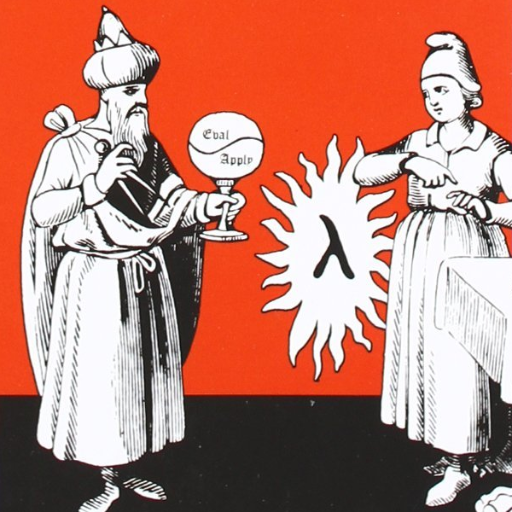
\includegraphics[width=0.8\paperwidth]{sicp.png}
      };
    \end{tikzpicture}
  \end{frame}
}

{ % all template changes are local to this group.
  \setbeamertemplate{navigation symbols}{}
  \begin{frame}[plain]
    \begin{tikzpicture}[remember picture,overlay]
      \node[at=(current page.center)] {
        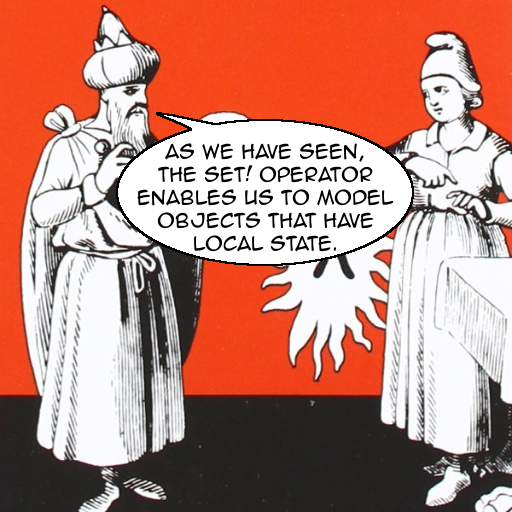
\includegraphics[width=0.8\paperwidth]{sicp1.png}
      };
    \end{tikzpicture}
  \end{frame}
}

{ % all template changes are local to this group.
  \setbeamertemplate{navigation symbols}{}
  \begin{frame}[plain]
    \begin{tikzpicture}[remember picture,overlay]
      \node[at=(current page.center)] {
        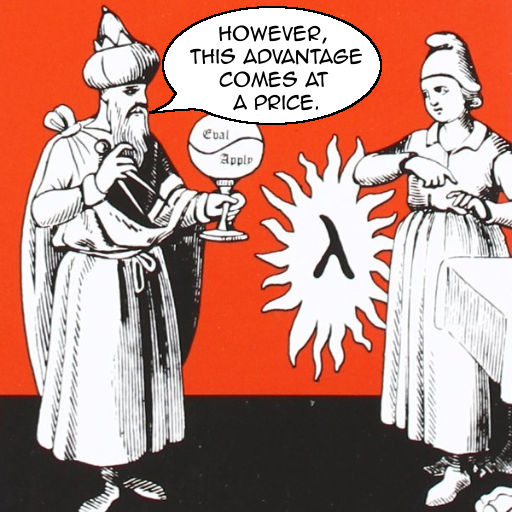
\includegraphics[width=0.8\paperwidth]{sicp2.png}
      };
    \end{tikzpicture}
  \end{frame}
}

{ % all template changes are local to this group.
  \setbeamertemplate{navigation symbols}{}
  \begin{frame}[plain]
    \begin{tikzpicture}[remember picture,overlay]
      \node[at=(current page.center)] {
        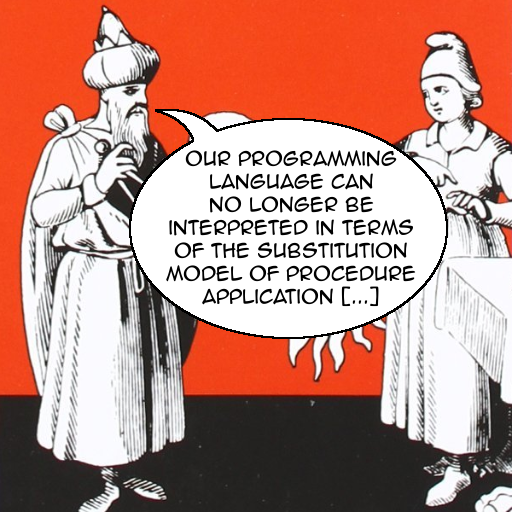
\includegraphics[width=0.8\paperwidth]{sicp3.png}
      };
    \end{tikzpicture}
  \end{frame}
}

{ % all template changes are local to this group.
  \setbeamertemplate{navigation symbols}{}
  \begin{frame}[plain]
    \begin{tikzpicture}[remember picture,overlay]
      \node[at=(current page.center)] {
        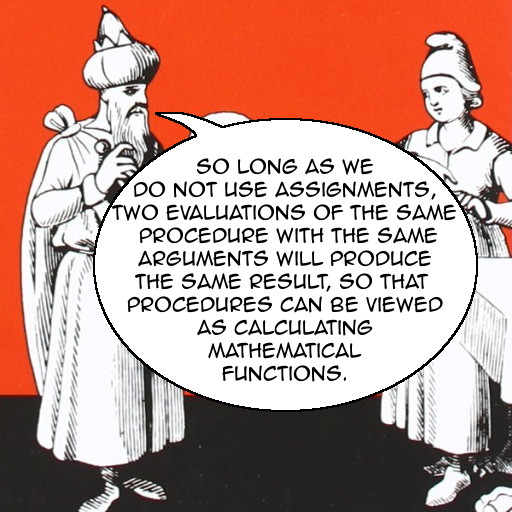
\includegraphics[width=0.8\paperwidth]{sicp4.png}
      };
    \end{tikzpicture}
  \end{frame}
}

{ % all template changes are local to this group.
  \setbeamertemplate{navigation symbols}{}
  \begin{frame}[plain]
    \begin{tikzpicture}[remember picture,overlay]
      \node[at=(current page.center)] {
        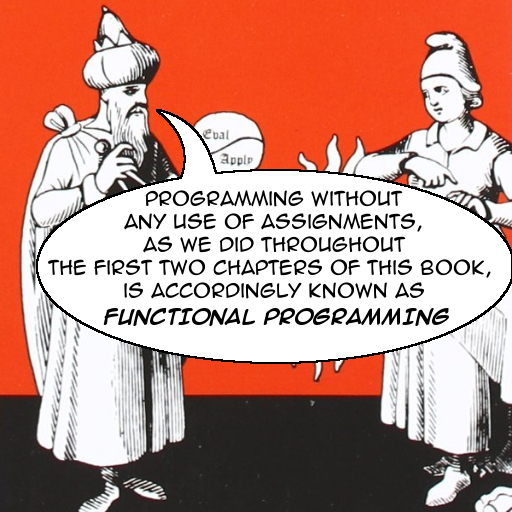
\includegraphics[width=0.8\paperwidth]{sicp5.png}
      };
    \end{tikzpicture}
  \end{frame}
}

{ % all template changes are local to this group.
  \setbeamertemplate{navigation symbols}{}
  \begin{frame}[plain]
    \begin{tikzpicture}[remember picture,overlay]
      \node[at=(current page.center)] {
        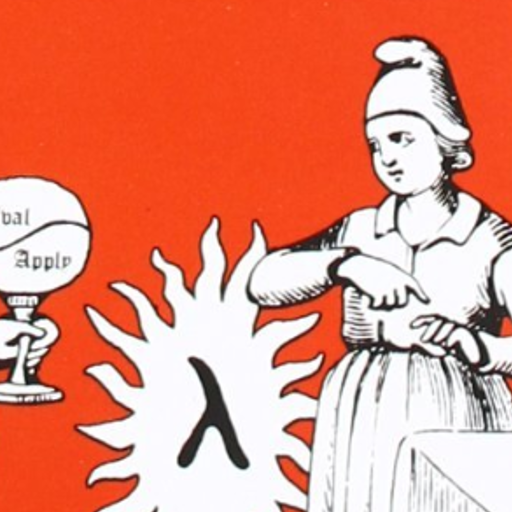
\includegraphics[width=0.8\paperwidth]{sicp6.png}
      };
    \end{tikzpicture}
  \end{frame}
}


%
\subsection{Referential opacity}

\begin{frame}{Referential opacity}
  \texttt{
    (define (compile expression result) \\*
    \ \ (match expression \\*
    \ \ \ \ (`(,<*> ,a ,b) \\*
    \ \ \ \ \ (let ((a+ (name a)) \\*
    \ \ \ \ \ \ \ \ \ \ \ (b+ (name b))) \\*
    \ \ \ \ \ \ \ `(,@(compile a a+)\\*
    \ \ \ \ \ \ \ \ \ ,@(compile b b+)\\*
    \ \ \ \ \ \ \ \ \ (,result = ,a+ ,<*> ,b+))))\\*
    \ \ \ \ (\_\\*
    \ \ \ \ \ '())))
  }
\end{frame}

\begin{frame}{Referential opacity}
  \texttt{
    (define (compile expression result) \\*
    \ \ (match expression \\*
    \ \ \ \ (\textbf{`(,<*> ,a ,b)} \\*
    \ \ \ \ \ (let ((a+ (name a)) \\*
    \ \ \ \ \ \ \ \ \ \ \ (b+ (name b))) \\*
    \ \ \ \ \ \ \ `(,@(compile a a+)\\*
    \ \ \ \ \ \ \ \ \ ,@(compile b b+)\\*
    \ \ \ \ \ \ \ \ \ (,result = ,a+ ,<*> ,b+))))\\*
    \ \ \ \ (\_\\*
    \ \ \ \ \ '())))
  }
\end{frame}

\begin{frame}{Referential opacity}
  \texttt{
    (define (compile expression result) \\*
    \ \ (match expression \\*
    \ \ \ \ (`(,<*> ,a ,b) \\*
    \ \ \ \ \ (let (\textbf{(a+ (name a)) \\*
    \ \ \ \ \ \ \ \ \ \ \ (b+ (name b))}) \\*
    \ \ \ \ \ \ \ `(,@(compile a a+)\\*
    \ \ \ \ \ \ \ \ \ ,@(compile b b+)\\*
    \ \ \ \ \ \ \ \ \ (,result = ,a+ ,<*> ,b+))))\\*
    \ \ \ \ (\_\\*
    \ \ \ \ \ '())))
  }
\end{frame}

\begin{frame}{Referential opacity}
  \texttt{
    (define (compile expression result) \\*
    \ \ (match expression \\*
    \ \ \ \ (`(,<*> ,a ,b) \\*
    \ \ \ \ \ (let ((a+ (name a)) \\*
    \ \ \ \ \ \ \ \ \ \ \ (b+ (name b))) \\*
    \ \ \ \ \ \ \ \textbf{`(,@(compile a a+)\\*
    \ \ \ \ \ \ \ \ \ ,@(compile b b+)\\*
    \ \ \ \ \ \ \ \ \ (,result = ,a+ ,<*> ,b+))}))\\*
    \ \ \ \ (\_\\*
    \ \ \ \ \ '())))
  }
\end{frame}

\begin{frame}{Referential opacity}
  \texttt{
    (define (compile expression result) \\*
    \ \ (match expression \\*
    \ \ \ \ (`(,<*> ,a ,b) \\*
    \ \ \ \ \ (let ((a+ (name a)) \\*
    \ \ \ \ \ \ \ \ \ \ \ (b+ (name b))) \\*
    \ \ \ \ \ \ \ `(,@(compile a a+)\\*
    \ \ \ \ \ \ \ \ \ ,@(compile b b+)\\*
    \ \ \ \ \ \ \ \ \ (,result = ,a+ ,<*> ,b+))))\\*
    \ \ \ \ \textbf{(\_\\*
    \ \ \ \ \ '())}))
  }
\end{frame}

\begin{frame}{Referential opacity}
  \texttt{
    (define name \\*
    \ \ (let ((counter 0)) \\*
    \ \ \ \ (lambda (expression)\\*
    \ \ \ \ \ \ (cond ((symbol? expression)\\*
    \ \ \ \ \ \ \ \ \ \ \ \ \ expression)\\*
    \ \ \ \ \ \ \ \ \ \ \ \ (else\\*
    \ \ \ \ \ \ \ \ \ \ \ \ \ (set! counter (+ counter 1))\\*
    \ \ \ \ \ \ \ \ \ \ \ \ \ (symbol-append 't\\*
    \ \ \ \ \ \ \ \ \ \ \ \ \ \ \ (number->symbol counter)))))))
  }
\end{frame}

\begin{frame}{Referential opacity}
  \texttt{
    (define name \\*
    \ \ (let (\textbf{(counter 0)}) \\*
    \ \ \ \ (lambda (expression)\\*
    \ \ \ \ \ \ (cond ((symbol? expression)\\*
    \ \ \ \ \ \ \ \ \ \ \ \ \ expression)\\*
    \ \ \ \ \ \ \ \ \ \ \ \ (else\\*
    \ \ \ \ \ \ \ \ \ \ \ \ \ (set! counter (+ counter 1))\\*
    \ \ \ \ \ \ \ \ \ \ \ \ \ (symbol-append 't\\*
    \ \ \ \ \ \ \ \ \ \ \ \ \ \ \ (number->symbol counter)))))))
  }
\end{frame}

\begin{frame}{Referential opacity}
  \texttt{
    (define name \\*
    \ \ (let ((counter 0)) \\*
    \ \ \ \ (lambda (expression)\\*
    \ \ \ \ \ \ (cond (\textbf{(symbol? expression)\\*
    \ \ \ \ \ \ \ \ \ \ \ \ \ expression})\\*
    \ \ \ \ \ \ \ \ \ \ \ \ (else\\*
    \ \ \ \ \ \ \ \ \ \ \ \ \ (set! counter (+ counter 1))\\*
    \ \ \ \ \ \ \ \ \ \ \ \ \ (symbol-append 't\\*
    \ \ \ \ \ \ \ \ \ \ \ \ \ \ \ (number->symbol counter)))))))
  }
\end{frame}

\begin{frame}{Referential opacity}
  \texttt{
    (define name \\*
    \ \ (let ((counter 0)) \\*
    \ \ \ \ (lambda (expression)\\*
    \ \ \ \ \ \ (cond ((symbol? expression)\\*
    \ \ \ \ \ \ \ \ \ \ \ \ \ expression)\\*
    \ \ \ \ \ \ \ \ \ \ \ \ (\textbf{else\\*
    \ \ \ \ \ \ \ \ \ \ \ \ \ (set! counter (+ counter 1))\\*
    \ \ \ \ \ \ \ \ \ \ \ \ \ (symbol-append 't\\*
    \ \ \ \ \ \ \ \ \ \ \ \ \ \ \ (number->symbol counter))})))))
  }
\end{frame}

\begin{frame}{Referential opacity}
  \texttt{(compile \textbf{'(* (+ x y) (/ z w)) 'result})\\*
    \ \\*
    \ \\*
    \ \\*
    \ \\*
    \ \\*
    \ \\*
    \ \\*
    \ }
\end{frame}

\begin{frame}{Referential opacity}
  \texttt{
    (match \textbf{'(* (+ x y) (/ z w))}\\*
    \ \ (`(,<*> ,a ,b)\\*
    \ \ \ (let ((a+ (name a))\\*
    \ \ \ \ \ \ \ \ \ (b+ (name b)))\\*
    \ \ \ \ \ `(,@(compile a a+)\\*
    \ \ \ \ \ \ \ ,@(compile b b+)\\*
    \ \ \ \ \ \ \ (\textbf{result} = ,a+ ,<*> ,b+))))\\*
    \ \ (\_\\*
    \ \ \ '()))
}
\end{frame}

\begin{frame}{Referential opacity}
  \texttt{
    (match '(\textbf{*} \textbf{(+ x y)} \textbf{(/ z w)})\\*
    \ \ (`(,\textbf{<*>} ,\textbf{a} ,\textbf{b})\\*
    \ \ \ (let ((a+ (name \textbf{a}))\\*
    \ \ \ \ \ \ \ \ \ (b+ (name \textbf{b})))\\*
    \ \ \ \ \ `(,@(compile \textbf{a} a+)\\*
    \ \ \ \ \ \ \ ,@(compile \textbf{b} b+)\\*
    \ \ \ \ \ \ \ (result = ,a+ ,\textbf{<*>} ,b+))))\\*
    \ \ (\_\\*
    \ \ \ '()))
}
\end{frame}

\begin{frame}{Referential opacity}
  \texttt{
    \ \\*
    \ \\*
    \ \ \ (let ((a+ (name \textbf{'(+ x y)}))\\*
    \ \ \ \ \ \ \ \ \ (b+ (name \textbf{'(/ z w)})))\\*
    \ \ \ \ \ `(,@(compile \textbf{'(+ x y)} a+)\\*
    \ \ \ \ \ \ \ ,@(compile \textbf{'(/ z w)} b+)\\*
    \ \ \ \ \ \ \ (result = ,a+ \textbf{*} ,b+))) \\*
    \ \\*
    \ 
  }
\end{frame}


\begin{frame}{Referential opacity}
  \texttt{
    \ \\*
    \ \\*
    \ \ \ (let ((a+ (name '(+ x y)))\\*
    \ \ \ \ \ \ \ \ \ (b+ (name '(/ z w))))\\*
    \ \ \ \ \ `(,@(compile '(+ x y) a+)\\*
    \ \ \ \ \ \ \ ,@(compile '(/ z w) b+)\\*
    \ \ \ \ \ \ \ (result = ,a+ * ,b+))) \\*
    \ \\*
    \ 
  }
\end{frame}

\begin{frame}{Referential opacity}
  \texttt{
    \ \\*
    \ \\*
    \ \ \ (let (\textbf{(a+ (name '(+ x y))) \\*
      \ \ \ \ \ \ \ \ \ (b+ (name '(/ z w)))})\\*
    \ \ \ \ \ `(,@(compile '(+ x y) a+)\\*
    \ \ \ \ \ \ \ ,@(compile '(/ z w) b+)\\*
    \ \ \ \ \ \ \ (result = ,a+ * ,b+))) \\*
    \ \\*
    \ 
  }
\end{frame}

\begin{frame}{Referential opacity}
  \texttt{
    \ \\*
    \ \\*
    \ \ \ (let (\textbf{(a+ 't1)\\*
      \ \ \ \ \ \ \ \ \  (b+ 't2)})\\*
    \ \ \ \ \ `(,@(compile '(+ x y) \textbf{a+})\\*
    \ \ \ \ \ \ \ ,@(compile '(/ z w) \textbf{b+})\\*
    \ \ \ \ \ \ \ (result = ,\textbf{a+} * ,\textbf{b+}))) \\*
    \ \\*
    \ 
  }
\end{frame}

\begin{frame}{Referential opacity}
  \texttt{
    \ \\*
    \ \\*
    \ \\*
    \ \\*
    \ \ \ \ \ `(,@(compile '(+ x y) \textbf{'t1})\\*
    \ \ \ \ \ \ \ ,@(compile '(/ z w) \textbf{'t2})\\*
    \ \ \ \ \ \ \ (result = \textbf{t1} * \textbf{t2})) \\*
    \ \\*
    \ 
  }
\end{frame}


\begin{frame}{Referential opacity}
  \texttt{
    \ \\*
    \ \\*
    \ \\*
    \ \\*
    \ \ \ \ \ `(,@\textbf{(compile '(+ x y) 't1)}\\*
    \ \ \ \ \ \ \ ,@\textbf{(compile '(/ z w) 't2)}\\*
    \ \ \ \ \ \ \ (result = t1 * t2)) \\*
    \ \\*
    \ 
  }
\end{frame}

\begin{frame}{Referential opacity}
  \texttt{
    \ \\*
    \ \\*
    \ \\*
    \ \\*
    \ \ \ \ \ '((t1 = x + y)\\*
    \ \ \ \ \ \ \ (t2 = z / w)\\*
    \ \ \ \ \ \ \ (result = t1 * t2)) \\*
    \ \\*
    \ 
  }
\end{frame}


%\subsection{Non-determinism}

\begin{frame}{Non-determinism}
  \texttt{
    (define (shuffle l)\\*
    \ \ (let ((n (length l)))\\*
    \ \ \ \ (if (is n < 2)\\*
    \ \ \ \ \ \ \ \ l\\*
    \ \ \ \ \ \ (let ((left right\\*
    \ \ \ \ \ \ \ \ \ \ \ \ \ \ \ \ \ \ (split-at l\\*
    \ \ \ \ \ \ \ \ \ \ \ \ \ \ \ \ \ \ \ \ \ (+ (random (- n 1))\\*
    \ \ \ \ \ \ \ \ \ \ \ \ \ \ \ \ \ \ \ \ \ \ \ \ 1))))\\*
    \ \ \ \ \ \ \ \ (if (= (random 2) 1)\\*
    \ \ \ \ \ \ \ \ \ \ \ \ `(,@(shuffle right)\\*
    \ \ \ \ \ \ \ \ \ \ \ \ \ \ ,@(shuffle left))\\*
    \ \ \ \ \ \ \ \ \ \ `(,@(shuffle left)\\*
    \ \ \ \ \ \ \ \ \ \ \ \ ,@(shuffle right)))))))
    }
\end{frame}

\begin{frame}{Non-determinism}
  \texttt{
    (define (shuffle l)\\*
    \ \ (let ((n (length l)))\\*
    \ \ \ \ (if \textbf{(is n < 2)\\*
    \ \ \ \ \ \ \ \ l}\\*
    \ \ \ \ \ \ (let ((left right\\*
    \ \ \ \ \ \ \ \ \ \ \ \ \ \ \ \ \ \ (split-at l\\*
    \ \ \ \ \ \ \ \ \ \ \ \ \ \ \ \ \ \ \ \ \ (+ (random (- n 1))\\*
    \ \ \ \ \ \ \ \ \ \ \ \ \ \ \ \ \ \ \ \ \ \ \ \ 1))))\\*
    \ \ \ \ \ \ \ \ (if (= (random 2) 1)\\*
    \ \ \ \ \ \ \ \ \ \ \ \ `(,@(shuffle right)\\*
    \ \ \ \ \ \ \ \ \ \ \ \ \ \ ,@(shuffle left))\\*
    \ \ \ \ \ \ \ \ \ \ `(,@(shuffle left)\\*
    \ \ \ \ \ \ \ \ \ \ \ \ ,@(shuffle right)))))))
    }
\end{frame}

\begin{frame}{Non-determinism}
  \texttt{
    (define (shuffle l)\\*
    \ \ (let ((n (length l)))\\*
    \ \ \ \ (if (is n < 2)\\*
    \ \ \ \ \ \ \ \ l\\*
    \ \ \ \ \ \ (let (\textbf{(left right\\*
    \ \ \ \ \ \ \ \ \ \ \ \ \ \ \ \ \ \ (split-at l\\*
    \ \ \ \ \ \ \ \ \ \ \ \ \ \ \ \ \ \ \ \ \ (+ (random (- n 1))\\*
    \ \ \ \ \ \ \ \ \ \ \ \ \ \ \ \ \ \ \ \ \ \ \ \ 1)))})\\*
    \ \ \ \ \ \ \ \ (if (= (random 2) 1)\\*
    \ \ \ \ \ \ \ \ \ \ \ \ `(,@(shuffle right)\\*
    \ \ \ \ \ \ \ \ \ \ \ \ \ \ ,@(shuffle left))\\*
    \ \ \ \ \ \ \ \ \ \ `(,@(shuffle left)\\*
    \ \ \ \ \ \ \ \ \ \ \ \ ,@(shuffle right)))))))
    }
\end{frame}


\begin{frame}{Non-determinism}
  \texttt{
    (define (shuffle l)\\*
    \ \ (let ((n (length l)))\\*
    \ \ \ \ (if (is n < 2)\\*
    \ \ \ \ \ \ \ \ l\\*
    \ \ \ \ \ \ (let ((left right\\*
    \ \ \ \ \ \ \ \ \ \ \ \ \ \ \ \ \ \ (split-at l\\*
    \ \ \ \ \ \ \ \ \ \ \ \ \ \ \ \ \ \ \ \ \ (+ (random (- n 1))\\*
    \ \ \ \ \ \ \ \ \ \ \ \ \ \ \ \ \ \ \ \ \ \ \ \ 1))))\\*
    \ \ \ \ \ \ \ \ (if \textbf{(= (random 2) 1)\\*
    \ \ \ \ \ \ \ \ \ \ \ \ `(,@(shuffle right)\\*
    \ \ \ \ \ \ \ \ \ \ \ \ \ \ ,@(shuffle left))}\\*
    \ \ \ \ \ \ \ \ \ \ `(,@(shuffle left)\\*
    \ \ \ \ \ \ \ \ \ \ \ \ ,@(shuffle right)))))))
    }
\end{frame}


\begin{frame}{Non-determinism}
  \texttt{
    (define (shuffle l)\\*
    \ \ (let ((n (length l)))\\*
    \ \ \ \ (if (is n < 2)\\*
    \ \ \ \ \ \ \ \ l\\*
    \ \ \ \ \ \ (let ((left right\\*
    \ \ \ \ \ \ \ \ \ \ \ \ \ \ \ \ \ \ (split-at l\\*
    \ \ \ \ \ \ \ \ \ \ \ \ \ \ \ \ \ \ \ \ \ (+ (random (- n 1))\\*
    \ \ \ \ \ \ \ \ \ \ \ \ \ \ \ \ \ \ \ \ \ \ \ \ 1))))\\*
    \ \ \ \ \ \ \ \ (if (= (random 2) 1)\\*
    \ \ \ \ \ \ \ \ \ \ \ \ `(,@(shuffle right)\\*
    \ \ \ \ \ \ \ \ \ \ \ \ \ \ ,@(shuffle left))\\*
    \ \ \ \ \ \ \ \ \ \ \textbf{`(,@(shuffle left)\\*
    \ \ \ \ \ \ \ \ \ \ \ \ ,@(shuffle right))})))))
    }
\end{frame}

\begin{frame}{Non-determinism}
  \texttt{
    (shuffle \textbf{'(a b c)})\\*
    \ \\*
    \ \\*
    \ \\*
    \ \\*
    \ \\*
    \ \\*
    \ \\*
    \ \\*
    \ \\*
    \ \\*
    \ \\*
    \ 
    }
\end{frame}

\begin{frame}{Non-determinism}
  \texttt{
    (let ((n (length \textbf{'(a b c)})))\\*
    \ \ (if (is n < 2)\\*
    \ \ \ \ \ \ \textbf{'(a b c)}\\*
    \ \ \ \ (let ((left right\\*
    \ \ \ \ \ \ \ \ \ \ \ \ \ \ \ \ (split-at \textbf{'(a b c)}\\*
    \ \ \ \ \ \ \ \ \ \ \ \ \ \ \ \ \ \ \ (+ (random (- n 1))\\*
    \ \ \ \ \ \ \ \ \ \ \ \ \ \ \ \ \ \ \ \ \ \ 1))))\\*
    \ \ \ \ \ \ (if (= (random 2) 1)\\*
    \ \ \ \ \ \ \ \ \ \ `(,@(shuffle right)\\*
    \ \ \ \ \ \ \ \ \ \ \ \ ,@(shuffle left))\\*
    \ \ \ \ \ \ \ \ `(,@(shuffle left)\\*
    \ \ \ \ \ \ \ \ \ \ ,@(shuffle right))))))\\*
    \ 
    }
\end{frame}


\begin{frame}{Non-determinism}
  \texttt{
    (let (\textbf{(n 3)})\\*
    \ \ (if (is \textbf{n} < 2)\\*
    \ \ \ \ \ \ '(a b c)\\*
    \ \ \ \ (let ((left right\\*
    \ \ \ \ \ \ \ \ \ \ \ \ \ \ \ \ (split-at '(a b c)\\*
    \ \ \ \ \ \ \ \ \ \ \ \ \ \ \ \ \ \ \ (+ (random (- \textbf{n} 1))\\*
    \ \ \ \ \ \ \ \ \ \ \ \ \ \ \ \ \ \ \ \ \ \ 1))))\\*
    \ \ \ \ \ \ (if (= (random 2) 1)\\*
    \ \ \ \ \ \ \ \ \ \ `(,@(shuffle right)\\*
    \ \ \ \ \ \ \ \ \ \ \ \ ,@(shuffle left))\\*
    \ \ \ \ \ \ \ \ `(,@(shuffle left)\\*
    \ \ \ \ \ \ \ \ \ \ ,@(shuffle right))))))\\*
    \ 
    }
\end{frame}


\begin{frame}{Non-determinism}
  \texttt{
    \ \\*
    \ \ (if (is \textbf{3} < 2)\\*
    \ \ \ \ \ \ '(a b c)\\*
    \ \ \ \ (let ((left right\\*
    \ \ \ \ \ \ \ \ \ \ \ \ \ \ \ \ (split-at '(a b c)\\*
    \ \ \ \ \ \ \ \ \ \ \ \ \ \ \ \ \ \ \ (+ (random (- \textbf{3} 1))\\*
    \ \ \ \ \ \ \ \ \ \ \ \ \ \ \ \ \ \ \ \ \ \ 1))))\\*
    \ \ \ \ \ \ (if (= (random 2) 1)\\*
    \ \ \ \ \ \ \ \ \ \ `(,@(shuffle right)\\*
    \ \ \ \ \ \ \ \ \ \ \ \ ,@(shuffle left))\\*
    \ \ \ \ \ \ \ \ `(,@(shuffle left)\\*
    \ \ \ \ \ \ \ \ \ \ ,@(shuffle right)))))\\*
    \ 
    }
\end{frame}

\begin{frame}{Non-determinism}
  \texttt{
    \ \\*
    \ \\*
    \ \\*
    \ \ \ \ (let ((left right\\*
    \ \ \ \ \ \ \ \ \ \ \ \ \ \ \ \ (split-at '(a b c)\\*
    \ \ \ \ \ \ \ \ \ \ \ \ \ \ \ \ \ \ \ (+ (random \textbf{2})\\*
    \ \ \ \ \ \ \ \ \ \ \ \ \ \ \ \ \ \ \ \ \ \ 1))))\\*
    \ \ \ \ \ \ (if (= (random 2) 1)\\*
    \ \ \ \ \ \ \ \ \ \ `(,@(shuffle right)\\*
    \ \ \ \ \ \ \ \ \ \ \ \ ,@(shuffle left))\\*
    \ \ \ \ \ \ \ \ `(,@(shuffle left)\\*
    \ \ \ \ \ \ \ \ \ \ ,@(shuffle right))))\\*
    \ 
    }
\end{frame}

\begin{frame}{Non-determinism}
  \texttt{
    \ \\*
    \ \\*
    \ \\*
    \ \ \ \ (let ((left right\\*
    \ \ \ \ \ \ \ \ \ \ \ \ \ \ \ \ (split-at '(a b c)\\*
    \ \ \ \ \ \ \ \ \ \ \ \ \ \ \ \ \ \ \ (+ \textbf{(random 2)}\\*
    \ \ \ \ \ \ \ \ \ \ \ \ \ \ \ \ \ \ \ \ \ \ 1))))\\*
    \ \ \ \ \ \ (if (= \textbf{(random 2)} 1)\\*
    \ \ \ \ \ \ \ \ \ \ `(,@(shuffle right)\\*
    \ \ \ \ \ \ \ \ \ \ \ \ ,@(shuffle left))\\*
    \ \ \ \ \ \ \ \ `(,@(shuffle left)\\*
    \ \ \ \ \ \ \ \ \ \ ,@(shuffle right))))\\*
    \ 
    }
\end{frame}

\begin{frame}{Non-determinism}
  \texttt{
    \ \\*
    \ \\*
    \ \ \ (let* (\textbf{\textcolor{red}{(x (random 2))}}\\*
    \ \ \ \ \ \ \ \ \ \ (left right\\*
    \ \ \ \ \ \ \ \ \ \ \ \ \ \ \ \ (split-at '(a b c)\\*
    \ \ \ \ \ \ \ \ \ \ \ \ \ \ \ \ \ \ \ (+ \textbf{\textcolor{red}{x}}\\*
    \ \ \ \ \ \ \ \ \ \ \ \ \ \ \ \ \ \ \ \ \ \ 1))))\\*
    \ \ \ \ \ \ (if (= \textbf{\textcolor{red}{x}} 1)\\*
    \ \ \ \ \ \ \ \ \ \ `(,@(shuffle right)\\*
    \ \ \ \ \ \ \ \ \ \ \ \ ,@(shuffle left))\\*
    \ \ \ \ \ \ \ \ `(,@(shuffle left)\\*
    \ \ \ \ \ \ \ \ \ \ ,@(shuffle right))))\\*
    \ 
    }
\end{frame}

\begin{frame}{Non-determinism}
  \texttt{
    \ \\*
    \ \\*
    \ \\*
    \ \ \ \ (let ((left right\\*
    \ \ \ \ \ \ \ \ \ \ \ \ \ \ \ \ (split-at '(a b c)\\*
    \ \ \ \ \ \ \ \ \ \ \ \ \ \ \ \ \ \ \ (+ \textbf{(random 2)}\\*
    \ \ \ \ \ \ \ \ \ \ \ \ \ \ \ \ \ \ \ \ \ \ 1))))\\*
    \ \ \ \ \ \ (if (= \textbf{(random 2)} 1)\\*
    \ \ \ \ \ \ \ \ \ \ `(,@(shuffle right)\\*
    \ \ \ \ \ \ \ \ \ \ \ \ ,@(shuffle left))\\*
    \ \ \ \ \ \ \ \ `(,@(shuffle left)\\*
    \ \ \ \ \ \ \ \ \ \ ,@(shuffle right))))\\*
    \ 
  }
\end{frame}

\begin{frame}{Non-determinism}
  \tiny
  \begin{tabularx}{\textwidth}{ X X }
    \texttt{(let ((left right (split-at '(a b c)\newline
      \hphantom{\_\_\_\_\_\_\_\_\_\_\_\_\_\_\_\_\_\_\_}
      (+ \textbf{(random 2)} 1))))\newline
      \hphantom{\_\_}(if (= \textbf{(random 2)} 1)\newline
      \hphantom{\_\_\_\_\_\_}`(,@(shuffle right)\newline
      \hphantom{ \_\_\_\_\_\_\_},@(shuffle left))\newline
      \hphantom{ \_\_\_\_}`(,@(shuffle left)\newline
      \hphantom{ \_\_\_\_\_\_},@(shuffle right))))\newline
      \ 
    }
    &
    \texttt{(let ((left right (split-at '(a b c)\newline
      \hphantom{\_\_\_\_\_\_\_\_\_\_\_\_\_\_\_\_\_\_\_}
      (+ \textbf{(random 2)} 1))))\newline
      \hphantom{\_\_}(if (= \textbf{(random 2)} 1)\newline
      \hphantom{\_\_\_\_\_\_}`(,@(shuffle right)\newline
      \hphantom{ \_\_\_\_\_\_\_},@(shuffle left))\newline
      \hphantom{ \_\_\_\_}`(,@(shuffle left)\newline
      \hphantom{ \_\_\_\_\_\_},@(shuffle right))))\newline
      \ 
    }

    \\
    
    \texttt{(let ((left right (split-at '(a b c)\newline
      \hphantom{\_\_\_\_\_\_\_\_\_\_\_\_\_\_\_\_\_\_\_}
      (+ \textbf{(random 2)} 1))))\newline
      \hphantom{\_\_}(if (= \textbf{(random 2)} 1)\newline
      \hphantom{\_\_\_\_\_\_}`(,@(shuffle right)\newline
      \hphantom{ \_\_\_\_\_\_\_},@(shuffle left))\newline
      \hphantom{ \_\_\_\_}`(,@(shuffle left)\newline
      \hphantom{ \_\_\_\_\_\_},@(shuffle right))))\newline
      \ 
    }
    &
    \texttt{(let ((left right (split-at '(a b c)\newline
      \hphantom{\_\_\_\_\_\_\_\_\_\_\_\_\_\_\_\_\_\_\_}
      (+ \textbf{(random 2)} 1))))\newline
      \hphantom{\_\_}(if (= \textbf{(random 2)} 1)\newline
      \hphantom{\_\_\_\_\_\_}`(,@(shuffle right)\newline
      \hphantom{ \_\_\_\_\_\_\_},@(shuffle left))\newline
      \hphantom{ \_\_\_\_}`(,@(shuffle left)\newline
      \hphantom{ \_\_\_\_\_\_},@(shuffle right))))\newline
      \ 
    }

  \end{tabularx}
\end{frame}


\begin{frame}{Non-determinism}
  \tiny
  \begin{tabularx}{\textwidth}{ X X }
    \texttt{(let ((left right (split-at '(a b c)\newline
      \hphantom{\_\_\_\_\_\_\_\_\_\_\_\_\_\_\_\_\_\_\_}
      (+ \textbf{0} 1))))\newline
      \hphantom{\_\_}(if (= \textbf{0} 1)\newline
      \hphantom{\_\_\_\_\_\_}`(,@(shuffle right)\newline
      \hphantom{ \_\_\_\_\_\_\_},@(shuffle left))\newline
      \hphantom{ \_\_\_\_}`(,@(shuffle left)\newline
      \hphantom{ \_\_\_\_\_\_},@(shuffle right))))\newline
      \ 
    }
    &
    \texttt{(let ((left right (split-at '(a b c)\newline
      \hphantom{\_\_\_\_\_\_\_\_\_\_\_\_\_\_\_\_\_\_\_}
      (+ \textbf{0} 1))))\newline
      \hphantom{\_\_}(if (= \textbf{1} 1)\newline
      \hphantom{\_\_\_\_\_\_}`(,@(shuffle right)\newline
      \hphantom{ \_\_\_\_\_\_\_},@(shuffle left))\newline
      \hphantom{ \_\_\_\_}`(,@(shuffle left)\newline
      \hphantom{ \_\_\_\_\_\_},@(shuffle right))))\newline
      \ 
    }

    \\
    
    \texttt{(let ((left right (split-at '(a b c)\newline
      \hphantom{\_\_\_\_\_\_\_\_\_\_\_\_\_\_\_\_\_\_\_}
      (+ \textbf{1} 1))))\newline
      \hphantom{\_\_}(if (= \textbf{0} 1)\newline
      \hphantom{\_\_\_\_\_\_}`(,@(shuffle right)\newline
      \hphantom{ \_\_\_\_\_\_\_},@(shuffle left))\newline
      \hphantom{ \_\_\_\_}`(,@(shuffle left)\newline
      \hphantom{ \_\_\_\_\_\_},@(shuffle right))))\newline
      \ 
    }
    &
    \texttt{(let ((left right (split-at '(a b c)\newline
      \hphantom{\_\_\_\_\_\_\_\_\_\_\_\_\_\_\_\_\_\_\_}
      (+ \textbf{1} 1))))\newline
      \hphantom{\_\_}(if (= \textbf{1} 1)\newline
      \hphantom{\_\_\_\_\_\_}`(,@(shuffle right)\newline
      \hphantom{ \_\_\_\_\_\_\_},@(shuffle left))\newline
      \hphantom{ \_\_\_\_}`(,@(shuffle left)\newline
      \hphantom{ \_\_\_\_\_\_},@(shuffle right))))\newline
      \ 
    }

  \end{tabularx}
\end{frame}


\begin{frame}{Non-determinism}
  \tiny
  \begin{tabularx}{\textwidth}{ X X }
    \texttt{(let ((left right (split-at '(a b c)\newline
      \hphantom{\_\_\_\_\_\_\_\_\_\_\_\_\_\_\_\_\_\_\_}
      \textbf{1})))\newline
      \hphantom{\_\_}(if \textbf{(= 0 1)}\newline
      \hphantom{\_\_\_\_\_\_}`(,@(shuffle right)\newline
      \hphantom{ \_\_\_\_\_\_\_},@(shuffle left))\newline
      \hphantom{ \_\_\_\_}\textbf{`(,@(shuffle left)\newline
      \hphantom{ \_\_\_\_\_\_},@(shuffle right))}))\newline
      \ 
    }
    &
    \texttt{(let ((left right (split-at '(a b c)\newline
      \hphantom{\_\_\_\_\_\_\_\_\_\_\_\_\_\_\_\_\_\_\_}
      \textbf{1})))\newline
      \hphantom{\_\_}(if \textbf{(= 1 1)}\newline
      \hphantom{\_\_\_\_\_\_}\textbf{`(,@(shuffle right)\newline
      \hphantom{ \_\_\_\_\_\_\_},@(shuffle left))}\newline
      \hphantom{ \_\_\_\_}`(,@(shuffle left)\newline
      \hphantom{ \_\_\_\_\_\_},@(shuffle right))))\newline
      \ 
    }

    \\
    
    \texttt{(let ((left right (split-at '(a b c)\newline
      \hphantom{\_\_\_\_\_\_\_\_\_\_\_\_\_\_\_\_\_\_\_}
      \textbf{2})))\newline
      \hphantom{\_\_}(if \textbf{(= 0 1)}\newline
      \hphantom{\_\_\_\_\_\_}`(,@(shuffle right)\newline
      \hphantom{ \_\_\_\_\_\_\_},@(shuffle left))\newline
      \hphantom{ \_\_\_\_}\textbf{`(,@(shuffle left)\newline
      \hphantom{ \_\_\_\_\_\_},@(shuffle right))}))\newline
      \ 
    }
    &
    \texttt{(let ((left right (split-at '(a b c)\newline
      \hphantom{\_\_\_\_\_\_\_\_\_\_\_\_\_\_\_\_\_\_\_}
      \textbf{2}))\newline
      \hphantom{\_\_}(if \textbf{(= 1 1)}\newline
      \hphantom{\_\_\_\_\_\_}\textbf{`(,@(shuffle right)\newline
      \hphantom{ \_\_\_\_\_\_\_},@(shuffle left))}\newline
      \hphantom{ \_\_\_\_}`(,@(shuffle left)\newline
      \hphantom{ \_\_\_\_\_\_},@(shuffle right))))\newline
      \ 
    }

  \end{tabularx}
\end{frame}



\begin{frame}{Non-determinism}
  \tiny
  \begin{tabularx}{\textwidth}{ X X }
    \texttt{\ \newline
      \ \newline
      \ \newline
      \ \newline
      \ \newline
      \hphantom{\_\_\_\_\_}\textbf{`(,@(shuffle '(a))\newline
      \hphantom{\_\_\_\_\_\_\_},@(shuffle '(b c)))}\newline
      \ 
    }
    &
    \texttt{\ \newline
      \ \newline
      \ \newline
      \hphantom{\_\_\_\_\_\_}\textbf{`(,@(shuffle '(b c))\newline
      \hphantom{\_\_\_\_\_\_\_\_},@(shuffle '(a)))}\newline
      \ \newline
      \ \newline
      \ 
    }

    \\

    \texttt{\ \newline
      \ \newline
      \ \newline
      \ \newline
      \ \newline
      \hphantom{\_\_\_\_\_}\textbf{`(,@(shuffle '(a b))\newline
      \hphantom{\_\_\_\_\_\_\_},@(shuffle '(c)))}\newline
      \ 
    }
    &
    \texttt{\ \newline
      \ \newline
      \ \newline
      \hphantom{\_\_\_\_\_\_}\textbf{`(,@(shuffle '(c))\newline
      \hphantom{\_\_\_\_\_\_\_\_},@(shuffle '(a b)))}\newline
      \ \newline
      \ \newline
      \ 
    }

  \end{tabularx}
\end{frame}



\begin{frame}{Non-determinism}
  \tiny
  \begin{tabularx}{\textwidth}{ X X }
    \texttt{\ \newline
      \ \newline
      \ \newline
      \ \newline
      \ \newline
      \hphantom{\_\_\_\_\_\_}\textbf{'(a b c)\newline
      \hphantom{\_\_\_\_\_\_}'(a c b)}\newline
      \ 
    }
    &
    \texttt{\ \newline
      \ \newline
      \ \newline
      \hphantom{\_\_\_\_\_\_}\textbf{'(b c a)\newline
      \hphantom{\_\_\_\_\_\_}'(c b a)}\newline
      \ \newline
      \ \newline
      \ 
    }

    \\

    \texttt{\ \newline
      \ \newline
      \ \newline
      \ \newline
      \ \newline
      \hphantom{\_\_\_\_\_\_}\textbf{'(a b c)\newline
      \hphantom{\_\_\_\_\_\_}'(b a c)}\newline
      \ 
    }
    &
    \texttt{\ \newline
      \ \newline
      \ \newline
      \hphantom{\_\_\_\_\_\_}\textbf{'(c a b)\newline
      \hphantom{\_\_\_\_\_\_}'(c b a)}\newline
      \ \newline
      \ \newline
      \ 
    }

  \end{tabularx}
\end{frame}

\begin{frame}{Non-determinism}
  \tiny
  \begin{tabularx}{\textwidth}{ X X }
    \texttt{\ \newline
      \ \newline
      \ \newline
      \ \newline
      \ \newline
      \hphantom{\_\_\_\_\_\_}\textbf{'(a b c)\newline
      \hphantom{\_\_\_\_\_\_}'(a c b)}\newline
      \ 
    }
    &
    \texttt{\ \newline
      \ \newline
      \ \newline
      \hphantom{\_\_\_\_\_\_}\textbf{'(b c a)\newline
      \hphantom{\_\_\_\_\_\_}'(c b a)}\newline
      \ \newline
      \ \newline
      \ 
    }

    \\

    \texttt{\ \newline
      \ \newline
      \ \newline
      \ \newline
      \ \newline
      \hphantom{\_\_\_\_\_\_}'(a b c)\newline
      \hphantom{\_\_\_\_\_\_}\textbf{'(b a c)}\newline
      \ 
    }
    &
    \texttt{\ \newline
      \ \newline
      \ \newline
      \hphantom{\_\_\_\_\_\_}\textbf{'(c a b)}\newline
      \hphantom{\_\_\_\_\_\_}'(c b a)\newline
      \ \newline
      \ \newline
      \ 
    }

  \end{tabularx}
\end{frame}


\subsection{Purity}

\begin{frame}{Purity}
\texttt{main :: IO () \\
main = do \{ \\ 
\ \ name <- getLine; \\ 
\ \ putStrLn "Hello "++name; \\
\} \\
  \
}
\end{frame}

\begin{frame}{FP vs OOP}
  \begin{center}
    \Huge
    \texttt{2 + 2} \\ \pause
  \end{center}
  \large
  \texttt{(+) :: Num a => a -> a -> a\\
    \ } \\ \pause
  \texttt{2.+(2)}
\end{frame}

\section{Object Oriented Programming}

\subsection{Definition}

%{ % all template changes are local to this group.
  \setbeamertemplate{navigation symbols}{}
  \begin{frame}[plain]
    \begin{tikzpicture}[remember picture,overlay]
      \node[at=(current page.center)] {
        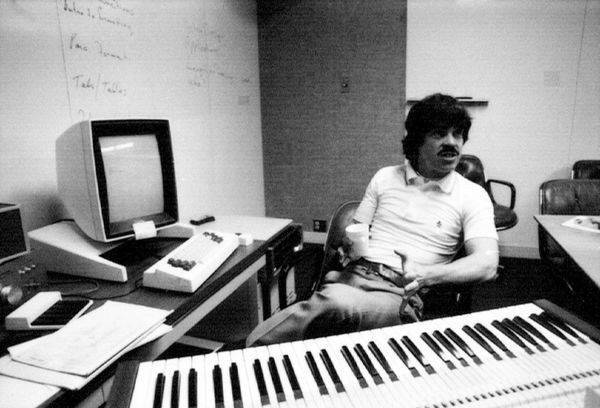
\includegraphics[height=\paperheight]{alan-kay.jpg}
      };
    \end{tikzpicture}
  \end{frame}
}

{ % all template changes are local to this group.
  \setbeamertemplate{navigation symbols}{}
  \begin{frame}[plain]
    \begin{tikzpicture}[remember picture,overlay]
      \node[at=(current page.center)] {
        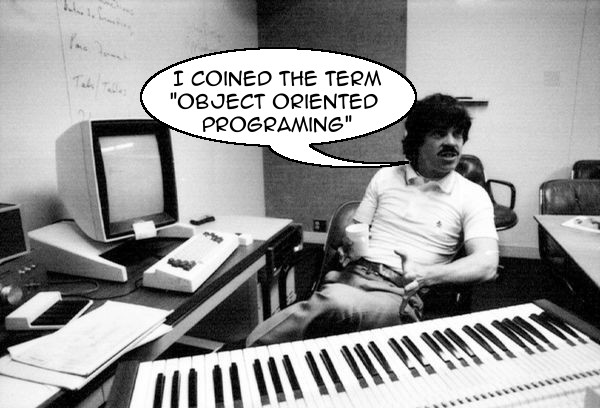
\includegraphics[height=\paperheight]{alan-kay-oop.jpg}
      };
    \end{tikzpicture}
  \end{frame}
}

{ % all template changes are local to this group.
  \setbeamertemplate{navigation symbols}{}
  \begin{frame}[plain]
    \begin{tikzpicture}[remember picture,overlay]
      \node[at=(current page.center)] {
        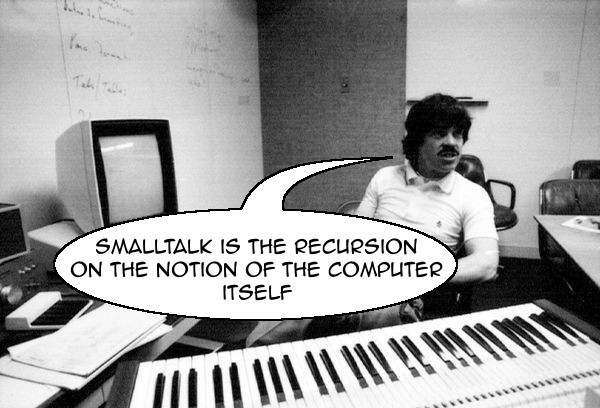
\includegraphics[height=\paperheight]{alan-kay-recomp.jpg}
      };
    \end{tikzpicture}
  \end{frame}
}

{ % all template changes are local to this group.
  \setbeamertemplate{navigation symbols}{}
  \begin{frame}[plain]
    \begin{tikzpicture}[remember picture,overlay]
      \node[at=(current page.center)] {
        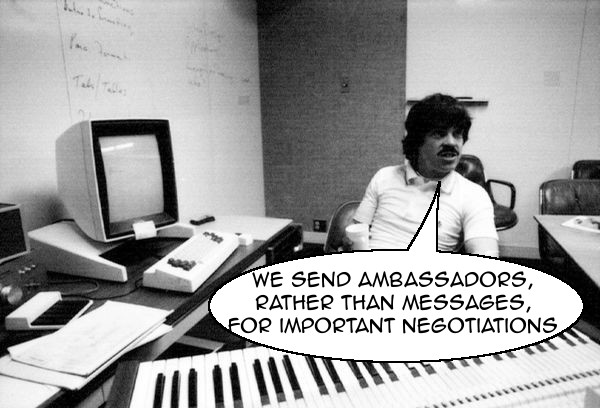
\includegraphics[height=\paperheight]{alan-kay-ambassadors.jpg}
      };
    \end{tikzpicture}
  \end{frame}
}


\begin{frame}{The notion of the computer (live demo)}
  \begin{center}
    \Huge
    \texttt{1.rkt}
  \end{center}
  \url{https://github.com/panicz/sracket}
\end{frame}

%\begin{frame}{The notion of the computer}
  \small
  \texttt{(define (draggable-rectangle left top width \\
    \ \ \ \ \ \ \ \ \ \ \ \ \ \ \ \ \ \ \ \ \ \ \ \ \ \ \ \ \ height color)\\
    \ (let ((dragged? \#false)\\
  \ \ \ \ \ \ \ (image (rectangle width height color)))\\
  \ \ \ \ (lambda message\\
  \ \ \ \ \ \ (match message\\
  \ \ \ \ \ \ \ \ (`(position) ...)\\
  \ \ \ \ \ \ \ \ (`(mouse-down ,x ,y) ...)\\
  \ \ \ \ \ \ \ \ (`(mouse-up ,x ,y) ...)\\
  \ \ \ \ \ \ \ \ (`(mouse-move ,x ,y ,dx ,dy) ...)\\
  \ \ \ \ \ \ \ \ (`(embraces? ,x ,y) ...)\\
  \ \ \ \ \ \ \ \ (`(as-image) ...)\\
  \ \ \ \ \ \ \ \ (`(mouse-out) ...)\\
  \ \ \ \ \ \ \ \ (\_ \#false)))))\\
  \ \\
  \ \\
  \ \\
  \ 
}
\end{frame}

\begin{frame}{The notion of the computer}
  \small
  \texttt{(define (draggable-rectangle \textbf{left top width \\
    \ \ \ \ \ \ \ \ \ \ \ \ \ \ \ \ \ \ \ \ \ \ \ \ \ \ \ \ \ height color})\\
    \ (let ((\textbf{dragged?} \#false)\\
  \ \ \ \ \ \ \ (\textbf{image} (rectangle width height color)))\\
  \ \ \ \ (lambda message\\
  \ \ \ \ \ \ (match message\\
  \ \ \ \ \ \ \ \ (`(position) ...)\\
  \ \ \ \ \ \ \ \ (`(mouse-down ,x ,y) ...)\\
  \ \ \ \ \ \ \ \ (`(mouse-up ,x ,y) ...)\\
  \ \ \ \ \ \ \ \ (`(mouse-move ,x ,y ,dx ,dy) ...)\\
  \ \ \ \ \ \ \ \ (`(embraces? ,x ,y) ...)\\
  \ \ \ \ \ \ \ \ (`(as-image) ...)\\
  \ \ \ \ \ \ \ \ (`(mouse-out) ...)\\
  \ \ \ \ \ \ \ \ (\_ \#false)))))\\
  \ \\
  \ \\
  \ \\
  \ 
}
\end{frame}

\begin{frame}{The notion of the computer}
  \small
  \texttt{(define (draggable-rectangle left top width \\
    \ \ \ \ \ \ \ \ \ \ \ \ \ \ \ \ \ \ \ \ \ \ \ \ \ \ \ \ \ height color)\\
    \ (let ((dragged? \#false)\\
  \ \ \ \ \ \ \ (image (rectangle width height color)))\\
  \ \ \ \ (lambda message\\
  \ \ \ \ \ \ (match message\\
  \ \ \ \ \ \ \ \ (\textbf{`(position) `(,left ,top)})\\
  \ \ \ \ \ \ \ \ (`(mouse-down ,x ,y) ...)\\
  \ \ \ \ \ \ \ \ (`(mouse-up ,x ,y) ...)\\
  \ \ \ \ \ \ \ \ (`(mouse-move ,x ,y ,dx ,dy) ...)\\
  \ \ \ \ \ \ \ \ (`(embraces? ,x ,y) ...)\\
  \ \ \ \ \ \ \ \ (`(as-image) ...)\\
  \ \ \ \ \ \ \ \ (`(mouse-out) ...)\\
  \ \ \ \ \ \ \ \ (\_ \#false)))))\\
  \ \\
  \ \\
  \ \\
  \ 
}
\end{frame}

\begin{frame}{The notion of the computer}
  \small
  \texttt{(define (draggable-rectangle left top width \\
    \ \ \ \ \ \ \ \ \ \ \ \ \ \ \ \ \ \ \ \ \ \ \ \ \ \ \ \ \ height color)\\
    \ (let ((dragged? \#false)\\
  \ \ \ \ \ \ \ (image (rectangle width height color)))\\
  \ \ \ \ (lambda message\\
  \ \ \ \ \ \ (match message\\
  \ \ \ \ \ \ \ \ (`(position) ...)\\
  \ \ \ \ \ \ \ \ (\textbf{`(mouse-down ,x ,y)\\
    \ \ \ \ \ \ \ \ \ (set! dragged? \#true)})\\
  \ \ \ \ \ \ \ \ (`(mouse-up ,x ,y) ...)\\
  \ \ \ \ \ \ \ \ (`(mouse-move ,x ,y ,dx ,dy) ...)\\
  \ \ \ \ \ \ \ \ (`(embraces? ,x ,y) ...)\\
  \ \ \ \ \ \ \ \ (`(as-image) ...)\\
  \ \ \ \ \ \ \ \ (`(mouse-out) ...)\\
  \ \ \ \ \ \ \ \ (\_ \#false)))))\\
  \ \\
  \ \\
  \ 
}
\end{frame}

\begin{frame}{The notion of the computer}
  \small
  \texttt{(define (draggable-rectangle left top width \\
    \ \ \ \ \ \ \ \ \ \ \ \ \ \ \ \ \ \ \ \ \ \ \ \ \ \ \ \ \ height color)\\
    \ (let ((dragged? \#false)\\
  \ \ \ \ \ \ \ (image (rectangle width height color)))\\
  \ \ \ \ (lambda message\\
  \ \ \ \ \ \ (match message\\
  \ \ \ \ \ \ \ \ (`(position) ...)\\
  \ \ \ \ \ \ \ \ (`(mouse-down ,x ,y) ...)\\
  \ \ \ \ \ \ \ \ (\textbf{`(mouse-up ,x ,y) \\
    \ \ \ \ \ \ \ \ \ (set! dragged? \#false)})\\
  \ \ \ \ \ \ \ \ (`(mouse-move ,x ,y ,dx ,dy) ...)\\
  \ \ \ \ \ \ \ \ (`(embraces? ,x ,y) ...)\\
  \ \ \ \ \ \ \ \ (`(as-image) ...)\\
  \ \ \ \ \ \ \ \ (`(mouse-out) ...)\\
  \ \ \ \ \ \ \ \ (\_ \#false)))))\\
  \ \\
  \ \\
  \ 
}
\end{frame}

\begin{frame}{The notion of the computer}
  \small
  \texttt{(define (draggable-rectangle left top width \\
    \ \ \ \ \ \ \ \ \ \ \ \ \ \ \ \ \ \ \ \ \ \ \ \ \ \ \ \ \ height color)\\
    \ (let ((dragged? \#false)\\
  \ \ \ \ \ \ \ (image (rectangle width height color)))\\
  \ \ \ \ (lambda message\\
  \ \ \ \ \ \ (match message\\
  \ \ \ \ \ \ \ \ (`(position) ...)\\
  \ \ \ \ \ \ \ \ (`(mouse-down ,x ,y) ...)\\
  \ \ \ \ \ \ \ \ (`(mouse-up ,x ,y) ...)\\
  \ \ \ \ \ \ \ \ (\textbf{`(mouse-move ,x ,y ,dx ,dy)\\
    \ \ \ \ \ \ \ \ \ (when dragged?\\
    \ \ \ \ \ \ \ \ \ \ \ (set! left (+ left dx)) \\  
    \ \ \ \ \ \ \ \ \ \ \ (set! top (+ top dy)))})\\
  \ \ \ \ \ \ \ \ (`(embraces? ,x ,y) ...)\\
  \ \ \ \ \ \ \ \ (`(as-image) ...)\\
  \ \ \ \ \ \ \ \ (`(mouse-out) ...)\\
  \ \ \ \ \ \ \ \ (\_ \#false)))))\\
  \ 
}
\end{frame}


\begin{frame}{The notion of the computer}
  \small
  \texttt{(define (draggable-rectangle left top width \\
    \ \ \ \ \ \ \ \ \ \ \ \ \ \ \ \ \ \ \ \ \ \ \ \ \ \ \ \ \ height color)\\
    \ (let ((dragged? \#false)\\
  \ \ \ \ \ \ \ (image (rectangle width height color)))\\
  \ \ \ \ (lambda message\\
  \ \ \ \ \ \ (match message\\
  \ \ \ \ \ \ \ \ (`(position) ...)\\
  \ \ \ \ \ \ \ \ (`(mouse-down ,x ,y) ...)\\
  \ \ \ \ \ \ \ \ (`(mouse-up ,x ,y) ...)\\
  \ \ \ \ \ \ \ \ (`(mouse-move ,x ,y ,dx ,dy) ...)\\
  \ \ \ \ \ \ \ \ (\textbf{`(embraces? ,x ,y) \\
    \ \ \ \ \ \ \ \ \ (and (is left <= x <= (+ left width))\\
    \ \ \ \ \ \ \ \ \ \ \ \ \ \ (is top <= y <= (+ top height)))})\\
  \ \ \ \ \ \ \ \ (`(as-image) ...)\\
  \ \ \ \ \ \ \ \ (`(mouse-out) ...)\\
  \ \ \ \ \ \ \ \ (\_ \#false)))))\\
  \ \\
  \ 
}
\end{frame}


\begin{frame}{The notion of the computer}
  \small
  \texttt{(define (draggable-rectangle left top width \\
    \ \ \ \ \ \ \ \ \ \ \ \ \ \ \ \ \ \ \ \ \ \ \ \ \ \ \ \ \ height color)\\
    \ (let ((dragged? \#false)\\
  \ \ \ \ \ \ \ (image (rectangle width height color)))\\
  \ \ \ \ (lambda message\\
  \ \ \ \ \ \ (match message\\
  \ \ \ \ \ \ \ \ (`(position) ...)\\
  \ \ \ \ \ \ \ \ (`(mouse-down ,x ,y) ...)\\
  \ \ \ \ \ \ \ \ (`(mouse-up ,x ,y) ...)\\
  \ \ \ \ \ \ \ \ (`(mouse-move ,x ,y ,dx ,dy) ...)\\
  \ \ \ \ \ \ \ \ (`(embraces? ,x ,y) ...)\\
  \ \ \ \ \ \ \ \ (\textbf{`(as-image) image})\\
  \ \ \ \ \ \ \ \ (`(mouse-out) ...)\\
  \ \ \ \ \ \ \ \ (\_ \#false)))))\\
  \ \\
  \ \\
  \ \\
  \ 
}
\end{frame}


\begin{frame}{The notion of the computer}
  \small
  \texttt{(define (draggable-rectangle left top width \\
    \ \ \ \ \ \ \ \ \ \ \ \ \ \ \ \ \ \ \ \ \ \ \ \ \ \ \ \ \ height color)\\
    \ (let ((dragged? \#false)\\
  \ \ \ \ \ \ \ (image (rectangle width height color)))\\
  \ \ \ \ (lambda message\\
  \ \ \ \ \ \ (match message\\
  \ \ \ \ \ \ \ \ (`(position) ...)\\
  \ \ \ \ \ \ \ \ (`(mouse-down ,x ,y) ...)\\
  \ \ \ \ \ \ \ \ (`(mouse-up ,x ,y) ...)\\
  \ \ \ \ \ \ \ \ (`(mouse-move ,x ,y ,dx ,dy) ...)\\
  \ \ \ \ \ \ \ \ (`(embraces? ,x ,y) ...)\\
  \ \ \ \ \ \ \ \ (`(as-image) ...)\\
  \ \ \ \ \ \ \ \ (\textbf{`(mouse-out) \\
  \ \ \ \ \ \ \ \ \ (set! dragged? \#false)})\\
  \ \ \ \ \ \ \ \ (\_ \#false)))))\\
  \ \\
  \ \\
  \ 
}
\end{frame}


\begin{frame}{The notion of the computer}
  \small
  \texttt{(define (draggable-rectangle left top width \\
    \ \ \ \ \ \ \ \ \ \ \ \ \ \ \ \ \ \ \ \ \ \ \ \ \ \ \ \ \ height color)\\
    \ (let ((dragged? \#false)\\
  \ \ \ \ \ \ \ (image (rectangle width height color)))\\
  \ \ \ \ (lambda message\\
  \ \ \ \ \ \ (match message\\
  \ \ \ \ \ \ \ \ (`(position) ...)\\
  \ \ \ \ \ \ \ \ (`(mouse-down ,x ,y) ...)\\
  \ \ \ \ \ \ \ \ (`(mouse-up ,x ,y) ...)\\
  \ \ \ \ \ \ \ \ (`(mouse-move ,x ,y ,dx ,dy) ...)\\
  \ \ \ \ \ \ \ \ (`(embraces? ,x ,y) ...)\\
  \ \ \ \ \ \ \ \ (`(as-image) ...)\\
  \ \ \ \ \ \ \ \ (`(mouse-out) ...)\\
  \ \ \ \ \ \ \ \ (\textbf{\_ \#false})))))\\
  \ \\
  \ \\
  \ \\
  \ 
}
\end{frame}

\begin{frame}{The notion of the computer}
  \scriptsize
  \texttt{(define stage\\
    \ \ (let* ((`(,width ,height) (screen-size))\\
    \ \ \ \ \ \ \ \ \ (elements ...)\\
    \ \ \ \ \ \ \ \ \ (image (rectangle width height 0))\\
    \ \ \ \ \ \ \ \ \ (hovered-element \#false))\\
    \ \ \ \ (lambda message\\
    \ \ \ \ \ \ (match message\\
    \ \ \ \ \ \ \ \ (`(as-image) ...)\\
    \ \ \ \ \ \ \ \ (`(mouse-down ,x ,y) ...)\\
    \ \ \ \ \ \ \ \ (`(mouse-up ,x ,y) ...)\\
    \ \ \ \ \ \ \ \ (`(mouse-move ,x ,y ,dx ,dy) ...)\\
    \ \ \ \ \ \ ))))\\
    \ \\
    \ \\
    \ \\
    \ \\
    \ \\
    \ \\
    \ \\
    \ \\
    \ \\
    \ \\
    \ 
}
\end{frame}

\begin{frame}{The notion of the computer}
  \scriptsize
  \texttt{(define stage\\
    \ \ (let* ((`(,width ,height) (screen-size))\\
    \ \ \ \ \ \ \ \ \ (\textbf{elements (map (lambda (\_)\\
      \ \ \ \ \ \ \ \ \ \ \ \ \ \ \ \ \ \ \ \ \ \ \ \ \ \ \ (draggable-rectangle\\
      \ \ \ \ \ \ \ \ \ \ \ \ \ \ \ \ \ \ \ \ \ \ \ \ \ \ \ \ \ (random (- width 50))\\
      \ \ \ \ \ \ \ \ \ \ \ \ \ \ \ \ \ \ \ \ \ \ \ \ \ \ \ \ \ (random (- height 50))\\
      \ \ \ \ \ \ \ \ \ \ \ \ \ \ \ \ \ \ \ \ \ \ \ \ \ \ \ \ \ 50 50 (random color)))\\
      \ \ \ \ \ \ \ \ \ \ \ \ \ \ \ \ \ \ \ \ \ \ \ \ (range 10))})\\
    \ \ \ \ \ \ \ \ \ (image (rectangle width height 0))\\
    \ \ \ \ \ \ \ \ \ (hovered-element \#false))\\
    \ \ \ \ (lambda message\\
    \ \ \ \ \ \ (match message\\
    \ \ \ \ \ \ \ \ (`(as-image) ...)\\
    \ \ \ \ \ \ \ \ (`(mouse-down ,x ,y) ...)\\
    \ \ \ \ \ \ \ \ (`(mouse-up ,x ,y) ...)\\
    \ \ \ \ \ \ \ \ (`(mouse-move ,x ,y ,dx ,dy) ...)\\
    \ \ \ \ \ \ ))))\\
    \ \\
    \ \\
    \ \\
    \ \\
    \ \\
    \ \\
    \ 
}
\end{frame}


\begin{frame}{The notion of the computer}
  \scriptsize
  \texttt{(define stage\\
    \ \ (let* ((`(,width ,height) (screen-size))\\
    \ \ \ \ \ \ \ \ \ (elements ...)\\
    \ \ \ \ \ \ \ \ \ (image (rectangle width height 0))\\
    \ \ \ \ \ \ \ \ \ (hovered-element \#false))\\
    \ \ \ \ (lambda message\\
    \ \ \ \ \ \ (match message\\
    \ \ \ \ \ \ \ \ (\textbf{`(as-image)\\
      \ \ \ \ \ \ \ \ \ (fill-image!\ image 0)\\
      \ \ \ \ \ \ \ \ \ (fold-right (lambda (e i)\\
      \ \ \ \ \ \ \ \ \ \ \ \ \ \ \ \ \ \ \ \ \ \ (let ((`(,x ,y) (e 'position)))\\
      \ \ \ \ \ \ \ \ \ \ \ \ \ \ \ \ \ \ \ \ \ \ \ \ (draw-image!\ (e 'as-image) x y i)\\
      \ \ \ \ \ \ \ \ \ \ \ \ \ \ \ \ \ \ \ \ \ \ \ \ i))\\
      \ \ \ \ \ \ \ \ \ \ \ \ \ \ \ \ \ \ \ \ \ image elements)\\
      \ \ \ \ \ \ \ \ \ image})\\
    \ \ \ \ \ \ \ \ (`(mouse-down ,x ,y) ...)\\
    \ \ \ \ \ \ \ \ (`(mouse-up ,x ,y) ...)\\
    \ \ \ \ \ \ \ \ (`(mouse-move ,x ,y ,dx ,dy) ...)\\
    \ \ \ \ \ \ ))))\\
    \ \\
    \ \\
    \ 
}
\end{frame}

\begin{frame}{The notion of the computer}
  \scriptsize
  \texttt{(define stage\\
    \ \ (let* ((`(,width ,height) (screen-size))\\
    \ \ \ \ \ \ \ \ \ (elements ...)\\
    \ \ \ \ \ \ \ \ \ (image (rectangle width height 0))\\
    \ \ \ \ \ \ \ \ \ (hovered-element \#false))\\
    \ \ \ \ (lambda message\\
    \ \ \ \ \ \ (match message\\
    \ \ \ \ \ \ \ \ (`(as-image) ...)\\
    \ \ \ \ \ \ \ \ (\textbf{`(mouse-down ,x ,y)\\
    \ \ \ \ \ \ \ \ \ (when hovered-element\\
    \ \ \ \ \ \ \ \ \ \ \ (hovered-element 'mouse-down x y))})\\
    \ \ \ \ \ \ \ \ (`(mouse-up ,x ,y) ...)\\
    \ \ \ \ \ \ \ \ (`(mouse-move ,x ,y ,dx ,dy) ...)\\
    \ \ \ \ \ \ ))))\\
    \ \\
    \ \\
    \ \\
    \ \\
    \ \\
    \ \\
    \ \\
    \ \\
    \ 
}
\end{frame}


\begin{frame}{The notion of the computer}
  \scriptsize
  \texttt{(define stage\\
    \ \ (let* ((`(,width ,height) (screen-size))\\
    \ \ \ \ \ \ \ \ \ (elements ...)\\
    \ \ \ \ \ \ \ \ \ (image (rectangle width height 0))\\
    \ \ \ \ \ \ \ \ \ (hovered-element \#false))\\
    \ \ \ \ (lambda message\\
    \ \ \ \ \ \ (match message\\
    \ \ \ \ \ \ \ \ (`(as-image) ...)\\
    \ \ \ \ \ \ \ \ (`(mouse-down ,x ,y) ...)\\
    \ \ \ \ \ \ \ \ (\textbf{`(mouse-up ,x ,y) \\
    \ \ \ \ \ \ \ \ \ (when hovered-element\\
    \ \ \ \ \ \ \ \ \ \ \ (hovered-element 'mouse-up x y))})\\
    \ \ \ \ \ \ \ \ (`(mouse-move ,x ,y ,dx ,dy) ...)\\
    \ \ \ \ \ \ ))))\\
    \ \\
    \ \\
    \ \\
    \ \\
    \ \\
    \ \\
    \ \\
    \ \\
    \ \\
    \ \\
    \ 
}
\end{frame}

\begin{frame}{The notion of the computer}
  \scriptsize
  \texttt{(define stage\\
    \ \ (let* ((`(,width ,height) (screen-size))\\
    \ \ \ \ \ \ \ \ \ (elements ...)\\
    \ \ \ \ \ \ \ \ \ (image (rectangle width height 0))\\
    \ \ \ \ \ \ \ \ \ (hovered-element \#false))\\
    \ \ \ \ (lambda message\\
    \ \ \ \ \ \ (match message\\
    \ \ \ \ \ \ \ \ (`(as-image) ...)\\
    \ \ \ \ \ \ \ \ (`(mouse-down ,x ,y) ...)\\
    \ \ \ \ \ \ \ \ (`(mouse-up ,x ,y) ...)\\
    \ \ \ \ \ \ \ \ (\textbf{`(mouse-move ,x ,y ,dx ,dy)\\
      \ \ \ \ \ \ \ \ \ (let ((hovered (find (lambda (\_)\\
      \ \ \ \ \ \ \ \ \ \ \ \ \ \ \ \ \ \ \ \ \ \ \ \ \ \ \ \ \ \ \ \ (\_ 'embraces? x y)) \\
      \ \ \ \ \ \ \ \ \ \ \ \ \ \ \ \ \ \ \ \ \ \ \ \ \ \ \ \ \ \ elements)))\\
    \ \ \ \ \ \ \ \ \ \ \ (unless (eq? hovered hovered-element)\\
    \ \ \ \ \ \ \ \ \ \ \ \ \ (when hovered-element (hovered-element 'mouse-out))\\
    \ \ \ \ \ \ \ \ \ \ \ \ \ (when hovered (hovered 'mouse-over))\\
    \ \ \ \ \ \ \ \ \ \ \ \ \ (set! hovered-element hovered))\\
    \ \ \ \ \ \ \ \ \ \ \ \ \ (when hovered (hovered 'mouse-move x y dx dy)))})\\
    \ \ \ \ \ \ ))))\\
    \ \\
    \ \\
    \ \\
    \ \\
    \ \\
    \ \\
    \ \\
    \ \\
    \ 
}
\end{frame}


\begin{frame}{Recursion on the notion of the computer (live demo)}
  \begin{center}
    \Huge
    \texttt{2.rkt}
  \end{center}
  \url{https://github.com/panicz/sracket}
\end{frame}

% 
\begin{frame}{Recursion on the notion of the computer}
  \tiny
  \texttt{(define (box \#:left left \#:top top \#:width width \#:height height\\
    \ \ \ \ \ \ \ \ \ \ \ \ \ \#:background-color color\\
    \ \ \ \ \ \ \ \ \ \ \ \ \ \#:draggable? [draggable? \#true] . elements)\\
    \ \ (let ((dragged? \#false)\\
    \ \ \ \ \ \ \ \ (hovered-element \#false)\\
    \ \ \ \ \ \ \ \ (image (rectangle width height color)))\\
    \ \ \ \ (lambda message\\
    \ \ \ \ \ \ (match message\\
    \ \ \ \ \ \ \ \ (`(position) ...)\\
    \ \ \ \ \ \ \ \ (`(mouse-down ,x ,y) ...)\\
    \ \ \ \ \ \ \ \ (`(mouse-up ,x ,y) ...)\\
    \ \ \ \ \ \ \ \ (`(mouse-move ,x ,y ,dx ,dy) ...)\\
    \ \ \ \ \ \ \ \ (`(embraces? ,x ,y) ...)\\
    \ \ \ \ \ \ \ \ (`(as-image) ...)\\
    \ \ \ \ \ \ \ \ (`(mouse-over) ...)\\
    \ \ \ \ \ \ \ \ (`(mouse-out) ...)))))\\
    \ \\
    \ \\
    \ \\
    \ \\
    \ \\
    \ \\
    \ \\
    \ \\
    \ \\
    \ \\
    \ \\
    \ 
    }
\end{frame}

\begin{frame}{Recursion on the notion of the computer}
  \tiny
  \texttt{(define (box \#:left left \#:top top \#:width width \#:height height\\
    \ \ \ \ \ \ \ \ \ \ \ \ \ \#:background-color \textbf{color}\\
    \ \ \ \ \ \ \ \ \ \ \ \ \ \#:draggable? [\textbf{draggable?} \#true] . \textbf{elements})\\
    \ \ (let ((dragged? \#false)\\
    \ \ \ \ \ \ \ \ (\textbf{hovered-element} \#false)\\
    \ \ \ \ \ \ \ \ (image (rectangle width height color)))\\
    \ \ \ \ (lambda message\\
    \ \ \ \ \ \ (match message\\
    \ \ \ \ \ \ \ \ (`(position) ...)\\
    \ \ \ \ \ \ \ \ (`(mouse-down ,x ,y) ...)\\
    \ \ \ \ \ \ \ \ (`(mouse-up ,x ,y) ...)\\
    \ \ \ \ \ \ \ \ (`(mouse-move ,x ,y ,dx ,dy) ...)\\
    \ \ \ \ \ \ \ \ (`(embraces? ,x ,y) ...)\\
    \ \ \ \ \ \ \ \ (`(as-image) ...)\\
    \ \ \ \ \ \ \ \ (`(mouse-over) ...)\\
    \ \ \ \ \ \ \ \ (`(mouse-out) ...)))))\\
    \ \\
    \ \\
    \ \\
    \ \\
    \ \\
    \ \\
    \ \\
    \ \\
    \ \\
    \ \\
    \ \\
    \ 
    }
\end{frame}

\begin{frame}{Recursion on the notion of the computer}
  \tiny
  \texttt{(define (box \#:left left \#:top top \#:width width \#:height height\\
    \ \ \ \ \ \ \ \ \ \ \ \ \ \#:background-color color\\
    \ \ \ \ \ \ \ \ \ \ \ \ \ \#:draggable? [draggable? \#true] . elements)\\
    \ \ (let ((dragged? \#false)\\
    \ \ \ \ \ \ \ \ (hovered-element \#false)\\
    \ \ \ \ \ \ \ \ (image (rectangle width height color)))\\
    \ \ \ \ (lambda message\\
    \ \ \ \ \ \ (match message\\
    \ \ \ \ \ \ \ \ (\textbf{`(position)} `(,left ,top))\\
    \ \ \ \ \ \ \ \ (`(mouse-down ,x ,y) ...)\\
    \ \ \ \ \ \ \ \ (`(mouse-up ,x ,y) ...)\\
    \ \ \ \ \ \ \ \ (`(mouse-move ,x ,y ,dx ,dy) ...)\\
    \ \ \ \ \ \ \ \ (`(embraces? ,x ,y) ...)\\
    \ \ \ \ \ \ \ \ (`(as-image) ...)\\
    \ \ \ \ \ \ \ \ (`(mouse-over) ...)\\
    \ \ \ \ \ \ \ \ (`(mouse-out) ...)))))\\
    \ \\
    \ \\
    \ \\
    \ \\
    \ \\
    \ \\
    \ \\
    \ \\
    \ \\
    \ \\
    \ \\
    \ 
    }
\end{frame}

\begin{frame}{Recursion on the notion of the computer}
  \tiny
  \texttt{(define (box \#:left left \#:top top \#:width width \#:height height\\
    \ \ \ \ \ \ \ \ \ \ \ \ \ \#:background-color color\\
    \ \ \ \ \ \ \ \ \ \ \ \ \ \#:draggable? [draggable? \#true] . elements)\\
    \ \ (let ((dragged? \#false)\\
    \ \ \ \ \ \ \ \ (hovered-element \#false)\\
    \ \ \ \ \ \ \ \ (image (rectangle width height color)))\\
    \ \ \ \ (lambda message\\
    \ \ \ \ \ \ (match message\\
    \ \ \ \ \ \ \ \ (`(position) ...)\\
    \ \ \ \ \ \ \ \ (\textbf{`(mouse-down ,x ,y)\\
      \ \ \ \ \ \ \ \ \ (if hovered-element\\
      \ \ \ \ \ \ \ \ \ \ \ \ (hovered-element 'mouse-down (- x left) (- y top))\\
      \ \ \ \ \ \ \ \ \ \ (when draggable?\\
      \ \ \ \ \ \ \ \ \ \ \ \ (set!\ dragged? \#true)))})\\
    \ \ \ \ \ \ \ \ (`(mouse-up ,x ,y) ...)\\
    \ \ \ \ \ \ \ \ (`(mouse-move ,x ,y ,dx ,dy) ...)\\
    \ \ \ \ \ \ \ \ (`(embraces? ,x ,y) ...)\\
    \ \ \ \ \ \ \ \ (`(as-image) ...)\\
    \ \ \ \ \ \ \ \ (`(mouse-over) ...)\\
    \ \ \ \ \ \ \ \ (`(mouse-out) ...)))))\\
    \ \\
    \ \\
    \ \\
    \ \\
    \ \\
    \ \\
    \ \\
    \ 
    }
\end{frame}

\begin{frame}{Recursion on the notion of the computer}
  \tiny
  \texttt{(define (box \#:left left \#:top top \#:width width \#:height height\\
    \ \ \ \ \ \ \ \ \ \ \ \ \ \#:background-color color\\
    \ \ \ \ \ \ \ \ \ \ \ \ \ \#:draggable? [draggable? \#true] . elements)\\
    \ \ (let ((dragged? \#false)\\
    \ \ \ \ \ \ \ \ (hovered-element \#false)\\
    \ \ \ \ \ \ \ \ (image (rectangle width height color)))\\
    \ \ \ \ (lambda message\\
    \ \ \ \ \ \ (match message\\
    \ \ \ \ \ \ \ \ (`(position) ...)\\
    \ \ \ \ \ \ \ \ (`(mouse-down ,x ,y) ...)\\
    \ \ \ \ \ \ \ \ (\textbf{`(mouse-up ,x ,y)\\
      \ \ \ \ \ \ \ \ \ (when hovered-element\\
      \ \ \ \ \ \ \ \ \ \ \ (hovered-element 'mouse-up (- x left) (- y top)))\\
      \ \ \ \ \ \ \ \ \ (set! dragged? \#false)})\\
    \ \ \ \ \ \ \ \ (`(mouse-move ,x ,y ,dx ,dy) ...)\\
    \ \ \ \ \ \ \ \ (`(embraces? ,x ,y) ...)\\
    \ \ \ \ \ \ \ \ (`(as-image) ...)\\
    \ \ \ \ \ \ \ \ (`(mouse-over) ...)\\
    \ \ \ \ \ \ \ \ (`(mouse-out) ...)))))\\
    \ \\
    \ \\
    \ \\
    \ \\
    \ \\
    \ \\
    \ \\
    \ \\
    \ 
    }
\end{frame}

\begin{frame}{Recursion on the notion of the computer}
  \tiny
  \texttt{(define (box \#:left left \#:top top \#:width width \#:height height\\
    \ \ \ \ \ \ \ \ \ \ \ \ \ \#:background-color color\\
    \ \ \ \ \ \ \ \ \ \ \ \ \ \#:draggable? [draggable? \#true] . elements)\\
    \ \ (let ((dragged? \#false)\\
    \ \ \ \ \ \ \ \ (hovered-element \#false)\\
    \ \ \ \ \ \ \ \ (image (rectangle width height color)))\\
    \ \ \ \ (lambda message\\
    \ \ \ \ \ \ (match message\\
    \ \ \ \ \ \ \ \ (`(position) ...)\\
    \ \ \ \ \ \ \ \ (`(mouse-down ,x ,y) ...)\\
    \ \ \ \ \ \ \ \ (`(mouse-up ,x ,y) ...)\\
    \ \ \ \ \ \ \ \ (\textbf{`(mouse-move ,x ,y ,dx ,dy)\\
      \ \ \ \ \ \ \ \ \ (cond (dragged?\\
      \ \ \ \ \ \ \ \ \ \ \ \ \ \ \ \ (set!\ left (+ left dx))\\
      \ \ \ \ \ \ \ \ \ \ \ \ \ \ \ \ (set!\ top (+ top dy)))\\
      \ \ \ \ \ \ \ \ \ \ \ \ \ \ \ (else\\
      \ \ \ \ \ \ \ \ \ \ \ \ \ \ \ \ (let ((hovered (find (\_ 'embraces?\ (- x left) (- y top))\\
      \ \ \ \ \ \ \ \ \ \ \ \ \ \ \ \ \ \ \ \ \ \ \ \ \ \ \ \ \ \ \ \ \ \ \ \ \ elements)))\\
      \ \ \ \ \ \ \ \ \ \ \ \ \ \ \ \ \ \ (unless (eq?\ hovered hovered-element)\\
      \ \ \ \ \ \ \ \ \ \ \ \ \ \ \ \ \ \ \ (when hovered-element (hovered-element 'mouse-out))\\
      \ \ \ \ \ \ \ \ \ \ \ \ \ \ \ \ \ \ \ (when hovered (hovered 'mouse-over))\\
      \ \ \ \ \ \ \ \ \ \ \ \ \ \ \ \ \ \ \ (set!\ hovered-element hovered))\\
      \ \ \ \ \ \ \ \ \ \ \ \ \ \ \ \ \ \ \ (when hovered \\
      \ \ \ \ \ \ \ \ \ \ \ \ \ \ \ \ \ \ \ \ \ (hovered 'mouse-move (- x left) (- y top) dx dy))))})\\
    \ \ \ \ \ \ \ \ (`(embraces? ,x ,y) ...)\\
    \ \ \ \ \ \ \ \ (`(as-image) ...)\\
    \ \ \ \ \ \ \ \ (`(mouse-over) ...)\\
    \ \ \ \ \ \ \ \ (`(mouse-out) ...)))))
    }
\end{frame}

\begin{frame}{Recursion on the notion of the computer}
  \tiny
  \texttt{(define (box \#:left left \#:top top \#:width width \#:height height\\
    \ \ \ \ \ \ \ \ \ \ \ \ \ \#:background-color color\\
    \ \ \ \ \ \ \ \ \ \ \ \ \ \#:draggable? [draggable? \#true] . elements)\\
    \ \ (let ((dragged? \#false)\\
    \ \ \ \ \ \ \ \ (hovered-element \#false)\\
    \ \ \ \ \ \ \ \ (image (rectangle width height color)))\\
    \ \ \ \ (lambda message\\
    \ \ \ \ \ \ (match message\\
    \ \ \ \ \ \ \ \ (`(position) ...)\\
    \ \ \ \ \ \ \ \ (`(mouse-down ,x ,y) ...)\\
    \ \ \ \ \ \ \ \ (`(mouse-up ,x ,y) ...)\\
    \ \ \ \ \ \ \ \ (`(mouse-move ,x ,y ,dx ,dy) ...)\\
    \ \ \ \ \ \ \ \ (\textbf{`(embraces? ,x ,y)\\
      \ \ \ \ \ \ \ \ \ (and (is left <= x <= (+ left width))\\
      \ \ \ \ \ \ \ \ \ \ \ \ \ \ (is top <= y <= (+ top height)))})\\
    \ \ \ \ \ \ \ \ (`(as-image) ...)\\
    \ \ \ \ \ \ \ \ (`(mouse-over) ...)\\
    \ \ \ \ \ \ \ \ (`(mouse-out) ...)))))\\
    \ \\
    \ \\
    \ \\
    \ \\
    \ \\
    \ \\
    \ \\
    \ \\
    \ \\
    \ 
    }
\end{frame}

\begin{frame}{Recursion on the notion of the computer}
  \tiny
  \texttt{(define (box \#:left left \#:top top \#:width width \#:height height\\
    \ \ \ \ \ \ \ \ \ \ \ \ \ \#:background-color color\\
    \ \ \ \ \ \ \ \ \ \ \ \ \ \#:draggable? [draggable? \#true] . elements)\\
    \ \ (let ((dragged? \#false)\\
    \ \ \ \ \ \ \ \ (hovered-element \#false)\\
    \ \ \ \ \ \ \ \ (image (rectangle width height color)))\\
    \ \ \ \ (lambda message\\
    \ \ \ \ \ \ (match message\\
    \ \ \ \ \ \ \ \ (`(position) ...)\\
    \ \ \ \ \ \ \ \ (`(mouse-down ,x ,y) ...)\\
    \ \ \ \ \ \ \ \ (`(mouse-up ,x ,y) ...)\\
    \ \ \ \ \ \ \ \ (`(mouse-move ,x ,y ,dx ,dy) ...)\\
    \ \ \ \ \ \ \ \ (`(embraces? ,x ,y) ...)\\
    \ \ \ \ \ \ \ \ (\textbf{`(as-image)\\
      \ \ \ \ \ \ \ \ \ (fill-image!\ image 0)\\
      \ \ \ \ \ \ \ \ \ (fold-right (lambda (e i)\\
      \ \ \ \ \ \ \ \ \ \ \ \ \ \ \ \ \ \ \ \ \ \ (let ((`(,x ,y) (e 'position)))\\
      \ \ \ \ \ \ \ \ \ \ \ \ \ \ \ \ \ \ \ \ \ \ \ \ (draw-image!\ (e 'as-image) x y i)\\
      \ \ \ \ \ \ \ \ \ \ \ \ \ \ \ \ \ \ \ \ \ \ \ \ i))\\
      \ \ \ \ \ \ \ \ \ \ \ \ \ \ \ \ \ \ \ \ \ image elements)\\
      \ \ \ \ \ \ \ \ \ image})\\
    \ \ \ \ \ \ \ \ (`(mouse-over) ...)\\
    \ \ \ \ \ \ \ \ (`(mouse-out) ...)))))\\
    \ \\
    \ \\
    \ \\
    \ \\
    \ 
  }
\end{frame}


\begin{frame}{Recursion on the notion of the computer}
  \tiny
  \texttt{(define (box \#:left left \#:top top \#:width width \#:height height\\
    \ \ \ \ \ \ \ \ \ \ \ \ \ \#:background-color color\\
    \ \ \ \ \ \ \ \ \ \ \ \ \ \#:draggable? [draggable? \#true] . elements)\\
    \ \ (let ((dragged? \#false)\\
    \ \ \ \ \ \ \ \ (hovered-element \#false)\\
    \ \ \ \ \ \ \ \ (image (rectangle width height color)))\\
    \ \ \ \ (lambda message\\
    \ \ \ \ \ \ (match message\\
    \ \ \ \ \ \ \ \ (`(position) ...)\\
    \ \ \ \ \ \ \ \ (`(mouse-down ,x ,y) ...)\\
    \ \ \ \ \ \ \ \ (`(mouse-up ,x ,y) ...)\\
    \ \ \ \ \ \ \ \ (`(mouse-move ,x ,y ,dx ,dy) ...)\\
    \ \ \ \ \ \ \ \ (`(embraces? ,x ,y) ...)\\
    \ \ \ \ \ \ \ \ (`(as-image) ...)\\
    \ \ \ \ \ \ \ \ (\textbf{`(mouse-over) \#false})\\
    \ \ \ \ \ \ \ \ (`(mouse-out) ...)))))\\
    \ \\
    \ \\
    \ \\
    \ \\
    \ \\
    \ \\
    \ \\
    \ \\
    \ \\
    \ \\
    \ \\
    \ 
    }
\end{frame}

\begin{frame}{Recursion on the notion of the computer}
  \tiny
  \texttt{(define (box \#:left left \#:top top \#:width width \#:height height\\
    \ \ \ \ \ \ \ \ \ \ \ \ \ \#:background-color color\\
    \ \ \ \ \ \ \ \ \ \ \ \ \ \#:draggable? [draggable? \#true] . elements)\\
    \ \ (let ((dragged? \#false)\\
    \ \ \ \ \ \ \ \ (hovered-element \#false)\\
    \ \ \ \ \ \ \ \ (image (rectangle width height color)))\\
    \ \ \ \ (lambda message\\
    \ \ \ \ \ \ (match message\\
    \ \ \ \ \ \ \ \ (`(position) ...)\\
    \ \ \ \ \ \ \ \ (`(mouse-down ,x ,y) ...)\\
    \ \ \ \ \ \ \ \ (`(mouse-up ,x ,y) ...)\\
    \ \ \ \ \ \ \ \ (`(mouse-move ,x ,y ,dx ,dy) ...)\\
    \ \ \ \ \ \ \ \ (`(embraces? ,x ,y) ...)\\
    \ \ \ \ \ \ \ \ (`(as-image) ...)\\
    \ \ \ \ \ \ \ \ (`(mouse-over) ...)\\
    \ \ \ \ \ \ \ \ (\textbf{`(mouse-out) (set!\ dragged?\ \#false)})))))\\
    \ \\
    \ \\
    \ \\
    \ \\
    \ \\
    \ \\
    \ \\
    \ \\
    \ \\
    \ \\
    \ \\
    \ 
    }
\end{frame}

\definecolor{topleftbox}{RGB}{119,204,0}
\definecolor{innertopleft}{RGB}{0,119,204}

\definecolor{innerbottomright}{RGB}{204,0,119}

\definecolor{bottomrightbox}{RGB}{119,0,204}

\definecolor{innerbottomright2}{RGB}{204,119,0}

\begin{frame}{Recursion on the notion of the computer}
  \scriptsize
  \texttt{\textbf{(define stage\\
    \ \ (let ((`(,w ,h) (screen-size)))\\
    \ \ \ \ (box \#:left 0 \#:top 0 \#:width w \#:height h\\
    \ \ \ \ \ \ \ \ \ \#:background-color \#x000000 \#:draggable?\ \#false\\
    \ \ \ \ \ \ \ \ \textcolor{topleftbox}{(box \#:left 10 \#:top 10 \#:width 200 \#:height 200\\
    \ \ \ \ \ \ \ \ \ \ \ \ \ \#:background-color \#x77cc00\\
    \ \ \ \ \ \ \ \ \ \ \ \ \textcolor{innertopleft}{(box \#:left 10 \#:top 10 \#:width 50 \#:height 50\\
    \ \ \ \ \ \ \ \ \ \ \ \ \ \ \ \ \ \#:background-color \#x0077cc\\
    \ \ \ \ \ \ \ \ \ \ \ \ \ \ \ \ \textcolor{red}{(box \#:left 5 \#:top 5 \#:width 20 \#:height 20\\
    \ \ \ \ \ \ \ \ \ \ \ \ \ \ \ \ \ \ \ \ \#:background-color \#xff0000)})}\\
    \ \ \ \ \ \ \ \ \ \ \ \ \textcolor{innerbottomright}{(box \#:left 140 \#:top 140 \#:width 50 \#:height 50\\
    \ \ \ \ \ \ \ \ \ \ \ \ \ \ \ \ \ \#:background-color \#xcc0077\\
    \ \ \ \ \ \ \ \ \ \ \ \ \ \ \ \ \ \#:draggable?\ \#false)})}\\
    \ \ \ \ \ \ \ \ \textcolor{bottomrightbox}{(box \#:left (- w 210) \#:top (- h 210) \\
    \ \ \ \ \ \ \ \ \ \ \ \ \ \#:width 200 \#:height 200\\
    \ \ \ \ \ \ \ \ \ \ \ \ \ \#:background-color \#x7700cc\\
    \ \ \ \ \ \ \ \ \ \ \ \ \textcolor{innerbottomright2}{(box \#:left 140 \#:top 140 \#:width 50 \#:height 50\\
    \ \ \ \ \ \ \ \ \ \ \ \ \ \ \ \ \ \#:background-color \#xcc7700)})})))}}
\end{frame}


\begin{frame}{Beyond the computer (live demo)}
  \begin{center}
    \Huge
    \texttt{3.rkt}
  \end{center}
  \url{https://github.com/panicz/sracket}
\end{frame}

%\begin{frame}{Beyond the computer}
  \tiny
  \texttt{(define (box \#:left left \#:top top \#:width width \#:height height\\
    \ \ \ \ \ \ \ \ \ \ \ \ \ \#:background-color color .\ elements)\\
    \ \ (let ((dragged-element \#false)\\
    \ \ \ \ \ \ \ \ (hovered-element \#false)\\
    \ \ \ \ \ \ \ \ (image (rectangle width height color)))\\
    \ \ \ \ (define (self .\ message)\\
    \ \ \ \ \ \ (match message\\
    \ \ \ \ \ \ \ \ (`(position) ...)\\
    \ \ \ \ \ \ \ \ (`(mouse-down ,x ,y) ...)\\
    \ \ \ \ \ \ \ \ (`(mouse-up ,x ,y) ...)\\
    \ \ \ \ \ \ \ \ (`(mouse-move ,x ,y ,dx ,dy) ...)\\
    \ \ \ \ \ \ \ \ (`(embraces?\ ,x ,y) ...)\\
    \ \ \ \ \ \ \ \ (`(as-image) ...)\\
    \ \ \ \ \ \ \ \ (`(move-by!\ ,dx ,dy) ...)\\
    \ \ \ \ \ \ \ \ (`(acquire-hovered-element!) ...)\\
    \ \ \ \ \ \ \ \ (`(install-element!\ ,element) ...)\\
    \ \ \ \ \ \ \ \ (\_ \#false)))\\
    \ \ \ \ self))} \\
  \ \\ \ \\ \ \\ \ \\ \ \\ \ \\ \ \\ \ \\ \ \\ \ \\ \ 
\end{frame}


\begin{frame}{Beyond the computer}
  \tiny
  \texttt{(define (box \#:left left \#:top top \#:width width \#:height height\\
    \ \ \ \ \ \ \ \ \ \ \ \ \ \#:background-color color .\ elements)\\
    \ \ (let ((\textbf{dragged-element} \#false)\\
    \ \ \ \ \ \ \ \ (hovered-element \#false)\\
    \ \ \ \ \ \ \ \ (image (rectangle width height color)))\\
    \ \ \ \ (define (self .\ message)\\
    \ \ \ \ \ \ (match message\\
    \ \ \ \ \ \ \ \ (`(position) ...)\\
    \ \ \ \ \ \ \ \ (`(mouse-down ,x ,y) ...)\\
    \ \ \ \ \ \ \ \ (`(mouse-up ,x ,y) ...)\\
    \ \ \ \ \ \ \ \ (`(mouse-move ,x ,y ,dx ,dy) ...)\\
    \ \ \ \ \ \ \ \ (`(embraces?\ ,x ,y) ...)\\
    \ \ \ \ \ \ \ \ (`(as-image) ...)\\
    \ \ \ \ \ \ \ \ (`(move-by!\ ,dx ,dy) ...)\\
    \ \ \ \ \ \ \ \ (`(acquire-hovered-element!) ...)\\
    \ \ \ \ \ \ \ \ (`(install-element!\ ,element) ...)\\
    \ \ \ \ \ \ \ \ (\_ \#false)))\\
    \ \ \ \ self))} \\
  \ \\ \ \\ \ \\ \ \\ \ \\ \ \\ \ \\ \ \\ \ \\ \ \\ \ 
\end{frame}

\begin{frame}{Beyond the computer}
  \tiny
  \texttt{(define (box \#:left left \#:top top \#:width width \#:height height\\
    \ \ \ \ \ \ \ \ \ \ \ \ \ \#:background-color color .\ elements)\\
    \ \ (let ((dragged-element \#false)\\
    \ \ \ \ \ \ \ \ (hovered-element \#false)\\
    \ \ \ \ \ \ \ \ (image (rectangle width height color)))\\
    \ \ \ \ (define (self .\ message)\\
    \ \ \ \ \ \ (match message\\
    \ \ \ \ \ \ \ \ (\textbf{`(position) `(,left ,top)})\\
    \ \ \ \ \ \ \ \ (`(mouse-down ,x ,y) ...)\\
    \ \ \ \ \ \ \ \ (`(mouse-up ,x ,y) ...)\\
    \ \ \ \ \ \ \ \ (`(mouse-move ,x ,y ,dx ,dy) ...)\\
    \ \ \ \ \ \ \ \ (`(embraces?\ ,x ,y) ...)\\
    \ \ \ \ \ \ \ \ (`(as-image) ...)\\
    \ \ \ \ \ \ \ \ (`(move-by!\ ,dx ,dy) ...)\\
    \ \ \ \ \ \ \ \ (`(acquire-hovered-element!) ...)\\
    \ \ \ \ \ \ \ \ (`(install-element!\ ,element) ...)\\
    \ \ \ \ \ \ \ \ (\_ \#false)))\\
    \ \ \ \ self))} \\
  \ \\ \ \\ \ \\ \ \\ \ \\ \ \\ \ \\ \ \\ \ \\ \ \\ \ 
\end{frame}

\begin{frame}{Beyond the computer}
  \tiny
  \texttt{(define (box \#:left left \#:top top \#:width width \#:height height\\
    \ \ \ \ \ \ \ \ \ \ \ \ \ \#:background-color color .\ elements)\\
    \ \ (let ((dragged-element \#false)\\
    \ \ \ \ \ \ \ \ (hovered-element \#false)\\
    \ \ \ \ \ \ \ \ (image (rectangle width height color)))\\
    \ \ \ \ (define (self .\ message)\\
    \ \ \ \ \ \ (match message\\
    \ \ \ \ \ \ \ \ (`(position) ...)\\
    \ \ \ \ \ \ \ \ (\textbf{`(mouse-down ,x ,y)\\
    \ \ \ \ \ \ \ \ \ (let ((acquired (self 'acquire-hovered-element!)))\\
    \ \ \ \ \ \ \ \ \ \ \ (when acquired\\
    \ \ \ \ \ \ \ \ \ \ \ \ \ (set!\ dragged-element acquired)))})\\
    \ \ \ \ \ \ \ \ (`(mouse-up ,x ,y) ...)\\
    \ \ \ \ \ \ \ \ (`(mouse-move ,x ,y ,dx ,dy) ...)\\
    \ \ \ \ \ \ \ \ (`(embraces?\ ,x ,y) ...)\\
    \ \ \ \ \ \ \ \ (`(as-image) ...)\\
    \ \ \ \ \ \ \ \ (`(move-by!\ ,dx ,dy) ...)\\
    \ \ \ \ \ \ \ \ (`(acquire-hovered-element!) ...)\\
    \ \ \ \ \ \ \ \ (`(install-element!\ ,element) ...)\\
    \ \ \ \ \ \ \ \ (\_ \#false)))\\
    \ \ \ \ self))} \\
  \ \\ \ \\ \ \\ \ \\ \ \\ \ \\ \ \\ \ 
\end{frame}

\begin{frame}{Beyond the computer}
  \tiny
  \texttt{(define (box \#:left left \#:top top \#:width width \#:height height\\
    \ \ \ \ \ \ \ \ \ \ \ \ \ \#:background-color color .\ elements)\\
    \ \ (let ((dragged-element \#false)\\
    \ \ \ \ \ \ \ \ (hovered-element \#false)\\
    \ \ \ \ \ \ \ \ (image (rectangle width height color)))\\
    \ \ \ \ (define (self .\ message)\\
    \ \ \ \ \ \ (match message\\
    \ \ \ \ \ \ \ \ (`(position) ...)\\
    \ \ \ \ \ \ \ \ (`(mouse-down ,x ,y) ...)\\
    \ \ \ \ \ \ \ \ (\textbf{`(mouse-up ,x ,y)\\
    \ \ \ \ \ \ \ \ \ (when dragged-element\\
    \ \ \ \ \ \ \ \ \ \ \ (self 'install-element!\ dragged-element)\\
    \ \ \ \ \ \ \ \ \ \ \ (set!\ dragged-element \#false))\\
    \ \ \ \ \ \ \ \ \ (self 'mouse-move x y 0 0)\\
    \ \ \ \ \ \ \ \ \ (when hovered-element\\
    \ \ \ \ \ \ \ \ \ \ \ (hovered-element 'mouse-up (- x left) (- y top)))})\\
    \ \ \ \ \ \ \ \ (`(mouse-up ,x ,y) ...)\\
    \ \ \ \ \ \ \ \ (`(mouse-move ,x ,y ,dx ,dy) ...)\\
    \ \ \ \ \ \ \ \ (`(embraces?\ ,x ,y) ...)\\
    \ \ \ \ \ \ \ \ (`(as-image) ...)\\
    \ \ \ \ \ \ \ \ (`(move-by!\ ,dx ,dy) ...)\\
    \ \ \ \ \ \ \ \ (`(acquire-hovered-element!) ...)\\
    \ \ \ \ \ \ \ \ (`(install-element!\ ,element) ...)\\
    \ \ \ \ \ \ \ \ (\_ \#false)))\\
    \ \ \ \ self))} \\
  \ \\ \ \\ \ \\ \ \\ \ 
\end{frame}

\begin{frame}{Beyond the computer}
  \tiny
  \texttt{(define (box \#:left left \#:top top \#:width width \#:height height\\
    \ \ \ \ \ \ \ \ \ \ \ \ \ \#:background-color color .\ elements)\\
    \ \ (let ((dragged-element \#false)\\
    \ \ \ \ \ \ \ \ (hovered-element \#false)\\
    \ \ \ \ \ \ \ \ (image (rectangle width height color)))\\
    \ \ \ \ (define (self .\ message)\\
    \ \ \ \ \ \ (match message\\
    \ \ \ \ \ \ \ \ (`(position) ...)\\
    \ \ \ \ \ \ \ \ (`(mouse-down ,x ,y) ...)\\
    \ \ \ \ \ \ \ \ (`(mouse-up ,x ,y) ...)\\
    \ \ \ \ \ \ \ \ (\textbf{`(mouse-move ,x ,y ,dx ,dy)\\
    \ \ \ \ \ \ \ \ \ (when dragged-element\\
    \ \ \ \ \ \ \ \ \ \ \ (dragged-element 'move-by!\ dx dy))\\
    \ \ \ \ \ \ \ \ \ (let ((hovered (find (\_ 'embraces?\ (- x left) (- y top))\\
    \ \ \ \ \ \ \ \ \ \ \ \ \ \ \ \ \ \ \ \ \ \ \ \ \ \ \ \ \ elements)))\\
    \ \ \ \ \ \ \ \ \ \ \ (unless (eq?\ hovered hovered-element)\\
    \ \ \ \ \ \ \ \ \ \ \ \ \ (when hovered-element\\
    \ \ \ \ \ \ \ \ \ \ \ \ \ \ \ (hovered-element 'mouse-out))\\
    \ \ \ \ \ \ \ \ \ \ \ \ \ (when hovered\\
    \ \ \ \ \ \ \ \ \ \ \ \ \ \ \ (hovered 'mouse-over))\\
    \ \ \ \ \ \ \ \ \ \ \ \ \ (set!\ hovered-element hovered))\\
    \ \ \ \ \ \ \ \ \ \ \ (when hovered\\
    \ \ \ \ \ \ \ \ \ \ \ \ \ (hovered 'mouse-move (- x left) (- y top) dx dy)))})\\
    \ \ \ \ \ \ \ \ (`(embraces?\ ,x ,y) ...)\\
    \ \ \ \ \ \ \ \ (`(as-image) ...)\\
    \ \ \ \ \ \ \ \ (`(move-by!\ ,dx ,dy) ...)\\
    \ \ \ \ \ \ \ \ (`(acquire-hovered-element!) ...)\\
    \ \ \ \ \ \ \ \ (`(install-element!\ ,element) ...)\\
    \ \ \ \ \ \ \ \ (\_ \#false)))\\
    \ \ \ \ self))}
\end{frame}

\begin{frame}{Beyond the computer}
  \tiny
  \texttt{(define (box \#:left left \#:top top \#:width width \#:height height\\
    \ \ \ \ \ \ \ \ \ \ \ \ \ \#:background-color color .\ elements)\\
    \ \ (let ((dragged-element \#false)\\
    \ \ \ \ \ \ \ \ (hovered-element \#false)\\
    \ \ \ \ \ \ \ \ (image (rectangle width height color)))\\
    \ \ \ \ (define (self .\ message)\\
    \ \ \ \ \ \ (match message\\
    \ \ \ \ \ \ \ \ (`(position) ...)\\
    \ \ \ \ \ \ \ \ (`(mouse-down ,x ,y) ...)\\
    \ \ \ \ \ \ \ \ (`(mouse-up ,x ,y) ...)\\
    \ \ \ \ \ \ \ \ (`(mouse-move ,x ,y ,dx ,dy) ...)\\
    \ \ \ \ \ \ \ \ (\textbf{`(embraces?\ ,x ,y)\\
    \ \ \ \ \ \ \ \ \ (and (is left <= x <= (+ left width))\\
    \ \ \ \ \ \ \ \ \ \ \ \ \ \ (is top <= y <= (+ top height)))})\\
    \ \ \ \ \ \ \ \ (`(as-image) ...)\\
    \ \ \ \ \ \ \ \ (`(move-by!\ ,dx ,dy) ...)\\
    \ \ \ \ \ \ \ \ (`(acquire-hovered-element!) ...)\\
    \ \ \ \ \ \ \ \ (`(install-element!\ ,element) ...)\\
    \ \ \ \ \ \ \ \ (\_ \#false)))\\
    \ \ \ \ self))} \\
  \ \\ \ \\ \ \\ \ \\ \ \\ \ \\ \ \\ \ \\ \ 
\end{frame}

\begin{frame}{Beyond the computer}
  \tiny
  \texttt{(define (box \#:left left \#:top top \#:width width \#:height height\\
    \ \ \ \ \ \ \ \ \ \ \ \ \ \#:background-color color .\ elements)\\
    \ \ (let ((dragged-element \#false)\\
    \ \ \ \ \ \ \ \ (hovered-element \#false)\\
    \ \ \ \ \ \ \ \ (image (rectangle width height color)))\\
    \ \ \ \ (define (self .\ message)\\
    \ \ \ \ \ \ (match message\\
    \ \ \ \ \ \ \ \ (`(position) ...)\\
    \ \ \ \ \ \ \ \ (`(mouse-down ,x ,y) ...)\\
    \ \ \ \ \ \ \ \ (`(mouse-up ,x ,y) ...)\\
    \ \ \ \ \ \ \ \ (`(mouse-move ,x ,y ,dx ,dy) ...)\\
    \ \ \ \ \ \ \ \ (`(embraces?\ ,x ,y) ...)\\
    \ \ \ \ \ \ \ \ (\textbf{`(as-image)\\
    \ \ \ \ \ \ \ \ \ (fill-image!\ image color)\\
    \ \ \ \ \ \ \ \ \ (fold-right (lambda (element image)\\
    \ \ \ \ \ \ \ \ \ \ \ \ \ \ \ \ \ \ \ \ \ \ \ (let ((`(,x ,y) (element 'position)))\\
    \ \ \ \ \ \ \ \ \ \ \ \ \ \ \ \ \ \ \ \ \ \ \ \ \ (draw-image!\ (element 'as-image) x y image)\\
    \ \ \ \ \ \ \ \ \ \ \ \ \ \ \ \ \ \ \ \ \ \ \ \ \ image))\\
    \ \ \ \ \ \ \ \ \ \ \ \ \ \ \ \ \ \ \ \ \ image\\
    \ \ \ \ \ \ \ \ \ \ \ \ \ \ \ \ \ \ \ \ \ `(,@(if dragged-element\\
    \ \ \ \ \ \ \ \ \ \ \ \ \ \ \ \ \ \ \ \ \ \ \ `(,dragged-element)\\
    \ \ \ \ \ \ \ \ \ \ \ \ \ \ \ \ \ \ \ \ \ \ \ '())\\
    \ \ \ \ \ \ \ \ \ \ \ \ \ \ \ \ \ \ \ \ \ \ ,@elements))})\\
    \ \ \ \ \ \ \ \ (`(move-by!\ ,dx ,dy) ...)\\
    \ \ \ \ \ \ \ \ (`(acquire-hovered-element!) ...)\\
    \ \ \ \ \ \ \ \ (`(install-element!\ ,element) ...)\\
    \ \ \ \ \ \ \ \ (\_ \#false)))\\
    \ \ \ \ self))} \\
  \ \\ \ \\ \ 
\end{frame}

\begin{frame}{Beyond the computer}
  \tiny
  \texttt{(define (box \#:left left \#:top top \#:width width \#:height height\\
    \ \ \ \ \ \ \ \ \ \ \ \ \ \#:background-color color .\ elements)\\
    \ \ (let ((dragged-element \#false)\\
    \ \ \ \ \ \ \ \ (hovered-element \#false)\\
    \ \ \ \ \ \ \ \ (image (rectangle width height color)))\\
    \ \ \ \ (define (self .\ message)\\
    \ \ \ \ \ \ (match message\\
    \ \ \ \ \ \ \ \ (`(position) ...)\\
    \ \ \ \ \ \ \ \ (`(mouse-down ,x ,y) ...)\\
    \ \ \ \ \ \ \ \ (`(mouse-up ,x ,y) ...)\\
    \ \ \ \ \ \ \ \ (`(mouse-move ,x ,y ,dx ,dy) ...)\\
    \ \ \ \ \ \ \ \ (`(embraces?\ ,x ,y) ...)\\
    \ \ \ \ \ \ \ \ (`(as-image) ...)\\
    \ \ \ \ \ \ \ \ (\textbf{`(move-by!\ ,dx ,dy)\\
    \ \ \ \ \ \ \ \ \ (set!\ left (+ left dx))\\
    \ \ \ \ \ \ \ \ \ (set!\ top (+ top dy))})\\
    \ \ \ \ \ \ \ \ (`(acquire-hovered-element!) ...)\\
    \ \ \ \ \ \ \ \ (`(install-element!\ ,element) ...)\\
    \ \ \ \ \ \ \ \ (\_ \#false)))\\
    \ \ \ \ self))} \\
  \ \\ \ \\ \ \\ \ \\ \ \\ \ \\ \ \\ \ \\ \ 
\end{frame}

\begin{frame}{Beyond the computer}
  \tiny
  \texttt{(define (box \#:left left \#:top top \#:width width \#:height height\\
    \ \ \ \ \ \ \ \ \ \ \ \ \ \#:background-color color .\ elements)\\
    \ \ (let ((dragged-element \#false)\\
    \ \ \ \ \ \ \ \ (hovered-element \#false)\\
    \ \ \ \ \ \ \ \ (image (rectangle width height color)))\\
    \ \ \ \ (define (self .\ message)\\
    \ \ \ \ \ \ (match message\\
    \ \ \ \ \ \ \ \ (`(position) ...)\\
    \ \ \ \ \ \ \ \ (`(mouse-down ,x ,y) ...)\\
    \ \ \ \ \ \ \ \ (`(mouse-up ,x ,y) ...)\\
    \ \ \ \ \ \ \ \ (`(mouse-move ,x ,y ,dx ,dy) ...)\\
    \ \ \ \ \ \ \ \ (`(embraces?\ ,x ,y) ...)\\
    \ \ \ \ \ \ \ \ (`(as-image) ...)\\
    \ \ \ \ \ \ \ \ (`(move-by!\ ,dx ,dy) ...)\\
    \ \ \ \ \ \ \ \ (\textbf{`(acquire-hovered-element!)\\
    \ \ \ \ \ \ \ \ \ (and hovered-element\\
    \ \ \ \ \ \ \ \ \ \ \ \ \ (or (and-let* ((acquired (hovered-element\\
    \ \ \ \ \ \ \ \ \ \ \ \ \ \ \ \ \ \ \ \ \ \ \ \ \ \ \ \ \ \ \ \ \ \ \ \ 'acquire-hovered-element!))\\
    \ \ \ \ \ \ \ \ \ \ \ \ \ \ \ \ \ \ \ \ \ \ \ \ \ \ \ \ \ (`(,x ,y) (hovered-element 'position)))\\
    \ \ \ \ \ \ \ \ \ \ \ \ \ \ \ \ \ \ \ \ \ \ \ \ \ \ (acquired 'move-by!\ x y)\\
    \ \ \ \ \ \ \ \ \ \ \ \ \ \ \ \ \ \ \ \ \ \ \ \ \ \ acquired)\\
    \ \ \ \ \ \ \ \ \ \ \ \ \ \ \ \ \ (let ((acquired hovered-element))\\
    \ \ \ \ \ \ \ \ \ \ \ \ \ \ \ \ \ \ \ (set!\ hovered-element \#false)\\
    \ \ \ \ \ \ \ \ \ \ \ \ \ \ \ \ \ \ \ (set!\ elements (filter (isnt \_ eq?\ acquired)\\
    \ \ \ \ \ \ \ \ \ \ \ \ \ \ \ \ \ \ \ \ \ \ \ \ \ \ \ \ \ \ \ \ \ \ \ elements))\\
    \ \ \ \ \ \ \ \ \ \ \ \ \ \ \ \ \ \ \ acquired)))})\\
    \ \ \ \ \ \ \ \ (`(install-element!\ ,element) ...)\\
    \ \ \ \ \ \ \ \ (\_ \#false)))\\
    \ \ \ \ self))}
\end{frame}

\begin{frame}{Beyond the computer}
  \tiny
  \texttt{(define (box \#:left left \#:top top \#:width width \#:height height\\
    \ \ \ \ \ \ \ \ \ \ \ \ \ \#:background-color color .\ elements)\\
    \ \ (let ((dragged-element \#false)\\
    \ \ \ \ \ \ \ \ (hovered-element \#false)\\
    \ \ \ \ \ \ \ \ (image (rectangle width height color)))\\
    \ \ \ \ (define (self .\ message)\\
    \ \ \ \ \ \ (match message\\
    \ \ \ \ \ \ \ \ (`(position) ...)\\
    \ \ \ \ \ \ \ \ (`(mouse-down ,x ,y) ...)\\
    \ \ \ \ \ \ \ \ (`(mouse-up ,x ,y) ...)\\
    \ \ \ \ \ \ \ \ (`(mouse-move ,x ,y ,dx ,dy) ...)\\
    \ \ \ \ \ \ \ \ (`(embraces?\ ,x ,y) ...)\\
    \ \ \ \ \ \ \ \ (`(as-image) ...)\\
    \ \ \ \ \ \ \ \ (`(move-by!\ ,dx ,dy) ...)\\
    \ \ \ \ \ \ \ \ (`(acquire-hovered-element!) ...)\\
    \ \ \ \ \ \ \ \ (\textbf{`(install-element!\ ,element)\\
    \ \ \ \ \ \ \ \ \ (if hovered-element\\
    \ \ \ \ \ \ \ \ \ \ \ \ (let ((`(,x ,y) (hovered-element 'position)))\\
    \ \ \ \ \ \ \ \ \ \ \ \ \ \ (element 'move-by!\ (- x) (- y))\\
    \ \ \ \ \ \ \ \ \ \ \ \ \ \ (hovered-element 'install-element!\ element))\\
    \ \ \ \ \ \ \ \ \ \ \ (set!\ elements `(,element .\ ,elements)))})\\
    \ \ \ \ \ \ \ \ (\_ \#false)))\\
    \ \ \ \ self))} \\
  \ \\ \ \\ \ \\ \ \\ \ \\ \ 
\end{frame}

\begin{frame}{Beyond the computer}
  \tiny
  \texttt{(define (box \#:left left \#:top top \#:width width \#:height height\\
    \ \ \ \ \ \ \ \ \ \ \ \ \ \#:background-color color .\ elements)\\
    \ \ (let ((dragged-element \#false)\\
    \ \ \ \ \ \ \ \ (hovered-element \#false)\\
    \ \ \ \ \ \ \ \ (image (rectangle width height color)))\\
    \ \ \ \ (define (self .\ message)\\
    \ \ \ \ \ \ (match message\\
    \ \ \ \ \ \ \ \ (`(position) ...)\\
    \ \ \ \ \ \ \ \ (`(mouse-down ,x ,y) ...)\\
    \ \ \ \ \ \ \ \ (`(mouse-up ,x ,y) ...)\\
    \ \ \ \ \ \ \ \ (`(mouse-move ,x ,y ,dx ,dy) ...)\\
    \ \ \ \ \ \ \ \ (`(embraces?\ ,x ,y) ...)\\
    \ \ \ \ \ \ \ \ (`(as-image) ...)\\
    \ \ \ \ \ \ \ \ (`(move-by!\ ,dx ,dy) ...)\\
    \ \ \ \ \ \ \ \ (`(acquire-hovered-element!) ...)\\
    \ \ \ \ \ \ \ \ (`(install-element!\ ,element) ...)\\
    \ \ \ \ \ \ \ \ (\textbf{\_ \#false})))\\
    \ \ \ \ self))} \\
  \ \\ \ \\ \ \\ \ \\ \ \\ \ \\ \ \\ \ \\ \ \\ \ \\ \ 
\end{frame}


%% \begin{frame}{Beyond the computer}
%%   \tiny
%%   \texttt{(define (box \#:left left \#:top top \#:width width \#:height height\\
%%     \ \ \ \ \ \ \ \ \ \ \ \ \ \#:background-color color .\ elements)\\
%%     \ \ (let ((dragged-element \#false)\\
%%     \ \ \ \ \ \ \ \ (hovered-element \#false)\\
%%     \ \ \ \ \ \ \ \ (image (rectangle width height color)))\\
%%     \ \ \ \ (define (self .\ message)\\
%%     \ \ \ \ \ \ (match message\\
%%     \ \ \ \ \ \ \ \ (`(position) `(,left ,top))\\
%%     \ \ \ \ \ \ \ \ (`(mouse-down ,x ,y)\\
%%     \ \ \ \ \ \ \ \ \ (let ((acquired (self 'acquire-hovered-element!)))\\
%%     \ \ \ \ \ \ \ \ \ \ \ (when acquired\\
%%     \ \ \ \ \ \ \ \ \ \ \ \ \ (set!\ dragged-element acquired))))\\
%%     \ \ \ \ \ \ \ \ (`(mouse-up ,x ,y)\\
%%     \ \ \ \ \ \ \ \ \ (when dragged-element\\
%%     \ \ \ \ \ \ \ \ \ \ \ (self 'install-element!\ dragged-element)\\
%%     \ \ \ \ \ \ \ \ \ \ \ (set!\ dragged-element \#false))\\
%%     \ \ \ \ \ \ \ \ \ (self 'mouse-move x y 0 0)\\
%%     \ \ \ \ \ \ \ \ \ (when hovered-element\\
%%     \ \ \ \ \ \ \ \ \ \ \ (hovered-element 'mouse-up (- x left) (- y top))))\\
%%     \ \ \ \ \ \ \ \ (`(mouse-move ,x ,y ,dx ,dy)\\
%%     \ \ \ \ \ \ \ \ \ (when dragged-element\\
%%     \ \ \ \ \ \ \ \ \ \ \ (dragged-element 'move-by!\ dx dy))\\
%%     \ \ \ \ \ \ \ \ \ (let ((hovered (find (\_ 'embraces?\ (- x left) (- y top))\\
%%     \ \ \ \ \ \ \ \ \ \ \ \ \ \ \ \ \ \ \ \ \ \ \ \ \ \ \ \ \ elements)))\\
%%     \ \ \ \ \ \ \ \ \ \ \ (unless (eq?\ hovered hovered-element)\\
%%     \ \ \ \ \ \ \ \ \ \ \ \ \ (when hovered-element\\
%%     \ \ \ \ \ \ \ \ \ \ \ \ \ \ \ (hovered-element 'mouse-out))\\
%%     \ \ \ \ \ \ \ \ \ \ \ \ \ (when hovered\\
%%     \ \ \ \ \ \ \ \ \ \ \ \ \ \ \ (hovered 'mouse-over))\\
%%     \ \ \ \ \ \ \ \ \ \ \ \ \ (set!\ hovered-element hovered))\\
%%     \ \ \ \ \ \ \ \ \ \ \ (when hovered\\
%%     \ \ \ \ \ \ \ \ \ \ \ \ \ (hovered 'mouse-move (- x left) (- y top) dx dy))))\\
%%     \ \ \ \ \ \ \ \ (`(embraces?\ ,x ,y)\\
%%     \ \ \ \ \ \ \ \ \ (and (is left <= x <= (+ left width))\\
%%     \ \ \ \ \ \ \ \ \ \ \ \ \ \ (is top <= y <= (+ top height))))\\
%%     \ \ \ \ \ \ \ \ (`(as-image)\\
%%     \ \ \ \ \ \ \ \ \ (fill-image!\ image color)\\
%%     \ \ \ \ \ \ \ \ \ (fold-right (lambda (element image)\\
%%     \ \ \ \ \ \ \ \ \ \ \ \ \ \ \ \ \ \ \ \ \ \ \ (let ((`(,x ,y) (element 'position)))\\
%%     \ \ \ \ \ \ \ \ \ \ \ \ \ \ \ \ \ \ \ \ \ \ \ \ \ (draw-image!\ (element 'as-image) x y image)\\
%%     \ \ \ \ \ \ \ \ \ \ \ \ \ \ \ \ \ \ \ \ \ \ \ \ \ image))\\
%%     \ \ \ \ \ \ \ \ \ \ \ \ \ \ \ \ \ \ \ \ \ image\\
%%     \ \ \ \ \ \ \ \ \ \ \ \ \ \ \ \ \ \ \ \ \ `(,@(if dragged-element\\
%%     \ \ \ \ \ \ \ \ \ \ \ \ \ \ \ \ \ \ \ \ \ \ \ `(,dragged-element)\\
%%     \ \ \ \ \ \ \ \ \ \ \ \ \ \ \ \ \ \ \ \ \ \ \ '())\\
%%     \ \ \ \ \ \ \ \ \ \ \ \ \ \ \ \ \ \ \ \ \ \ ,@elements)))\\
%%     \ \ \ \ \ \ \ \ (`(move-by!\ ,dx ,dy)\\
%%     \ \ \ \ \ \ \ \ \ (set!\ left (+ left dx))\\
%%     \ \ \ \ \ \ \ \ \ (set!\ top (+ top dy)))\\
%%     \ \ \ \ \ \ \ \ (`(acquire-hovered-element!)\\
%%     \ \ \ \ \ \ \ \ \ (and hovered-element\\
%%     \ \ \ \ \ \ \ \ \ \ \ \ \ (or (and-let* ((acquired (hovered-element\\
%%     \ \ \ \ \ \ \ \ \ \ \ \ \ \ \ \ \ \ \ \ \ \ \ \ \ \ \ \ \ \ \ \ \ \ \ \ 'acquire-hovered-element!))\\
%%     \ \ \ \ \ \ \ \ \ \ \ \ \ \ \ \ \ \ \ \ \ \ \ \ \ \ \ \ \ (`(,x ,y) (hovered-element 'position)))\\
%%     \ \ \ \ \ \ \ \ \ \ \ \ \ \ \ \ \ \ \ \ \ \ \ \ \ \ (acquired 'move-by!\ x y)\\
%%     \ \ \ \ \ \ \ \ \ \ \ \ \ \ \ \ \ \ \ \ \ \ \ \ \ \ acquired)\\
%%     \ \ \ \ \ \ \ \ \ \ \ \ \ \ \ \ \ (let ((acquired hovered-element))\\
%%     \ \ \ \ \ \ \ \ \ \ \ \ \ \ \ \ \ \ \ (set!\ hovered-element \#false)\\
%%     \ \ \ \ \ \ \ \ \ \ \ \ \ \ \ \ \ \ \ (set!\ elements (filter (isnt \_ eq?\ acquired)\\
%%     \ \ \ \ \ \ \ \ \ \ \ \ \ \ \ \ \ \ \ \ \ \ \ \ \ \ \ \ \ \ \ \ \ \ \ elements))\\
%%     \ \ \ \ \ \ \ \ \ \ \ \ \ \ \ \ \ \ \ acquired))))\\
%%     \ \ \ \ \ \ \ \ (`(install-element!\ ,element)\\
%%     \ \ \ \ \ \ \ \ \ (if hovered-element\\
%%     \ \ \ \ \ \ \ \ \ \ \ \ (let ((`(,x ,y) (hovered-element 'position)))\\
%%     \ \ \ \ \ \ \ \ \ \ \ \ \ \ (element 'move-by!\ (- x) (- y))\\
%%     \ \ \ \ \ \ \ \ \ \ \ \ \ \ (hovered-element 'install-element!\ element))\\
%%     \ \ \ \ \ \ \ \ \ \ \ (set!\ elements `(,element .\ ,elements))))\\
%%     \ \ \ \ \ \ \ \ (\_ \#false)))\\
%%     \ \ \ \ self))}
%% \end{frame}


{ % all template changes are local to this group.
  \setbeamertemplate{navigation symbols}{}
  \begin{frame}[plain]
    \begin{tikzpicture}[remember picture,overlay]
      \node[at=(current page.center)] {
        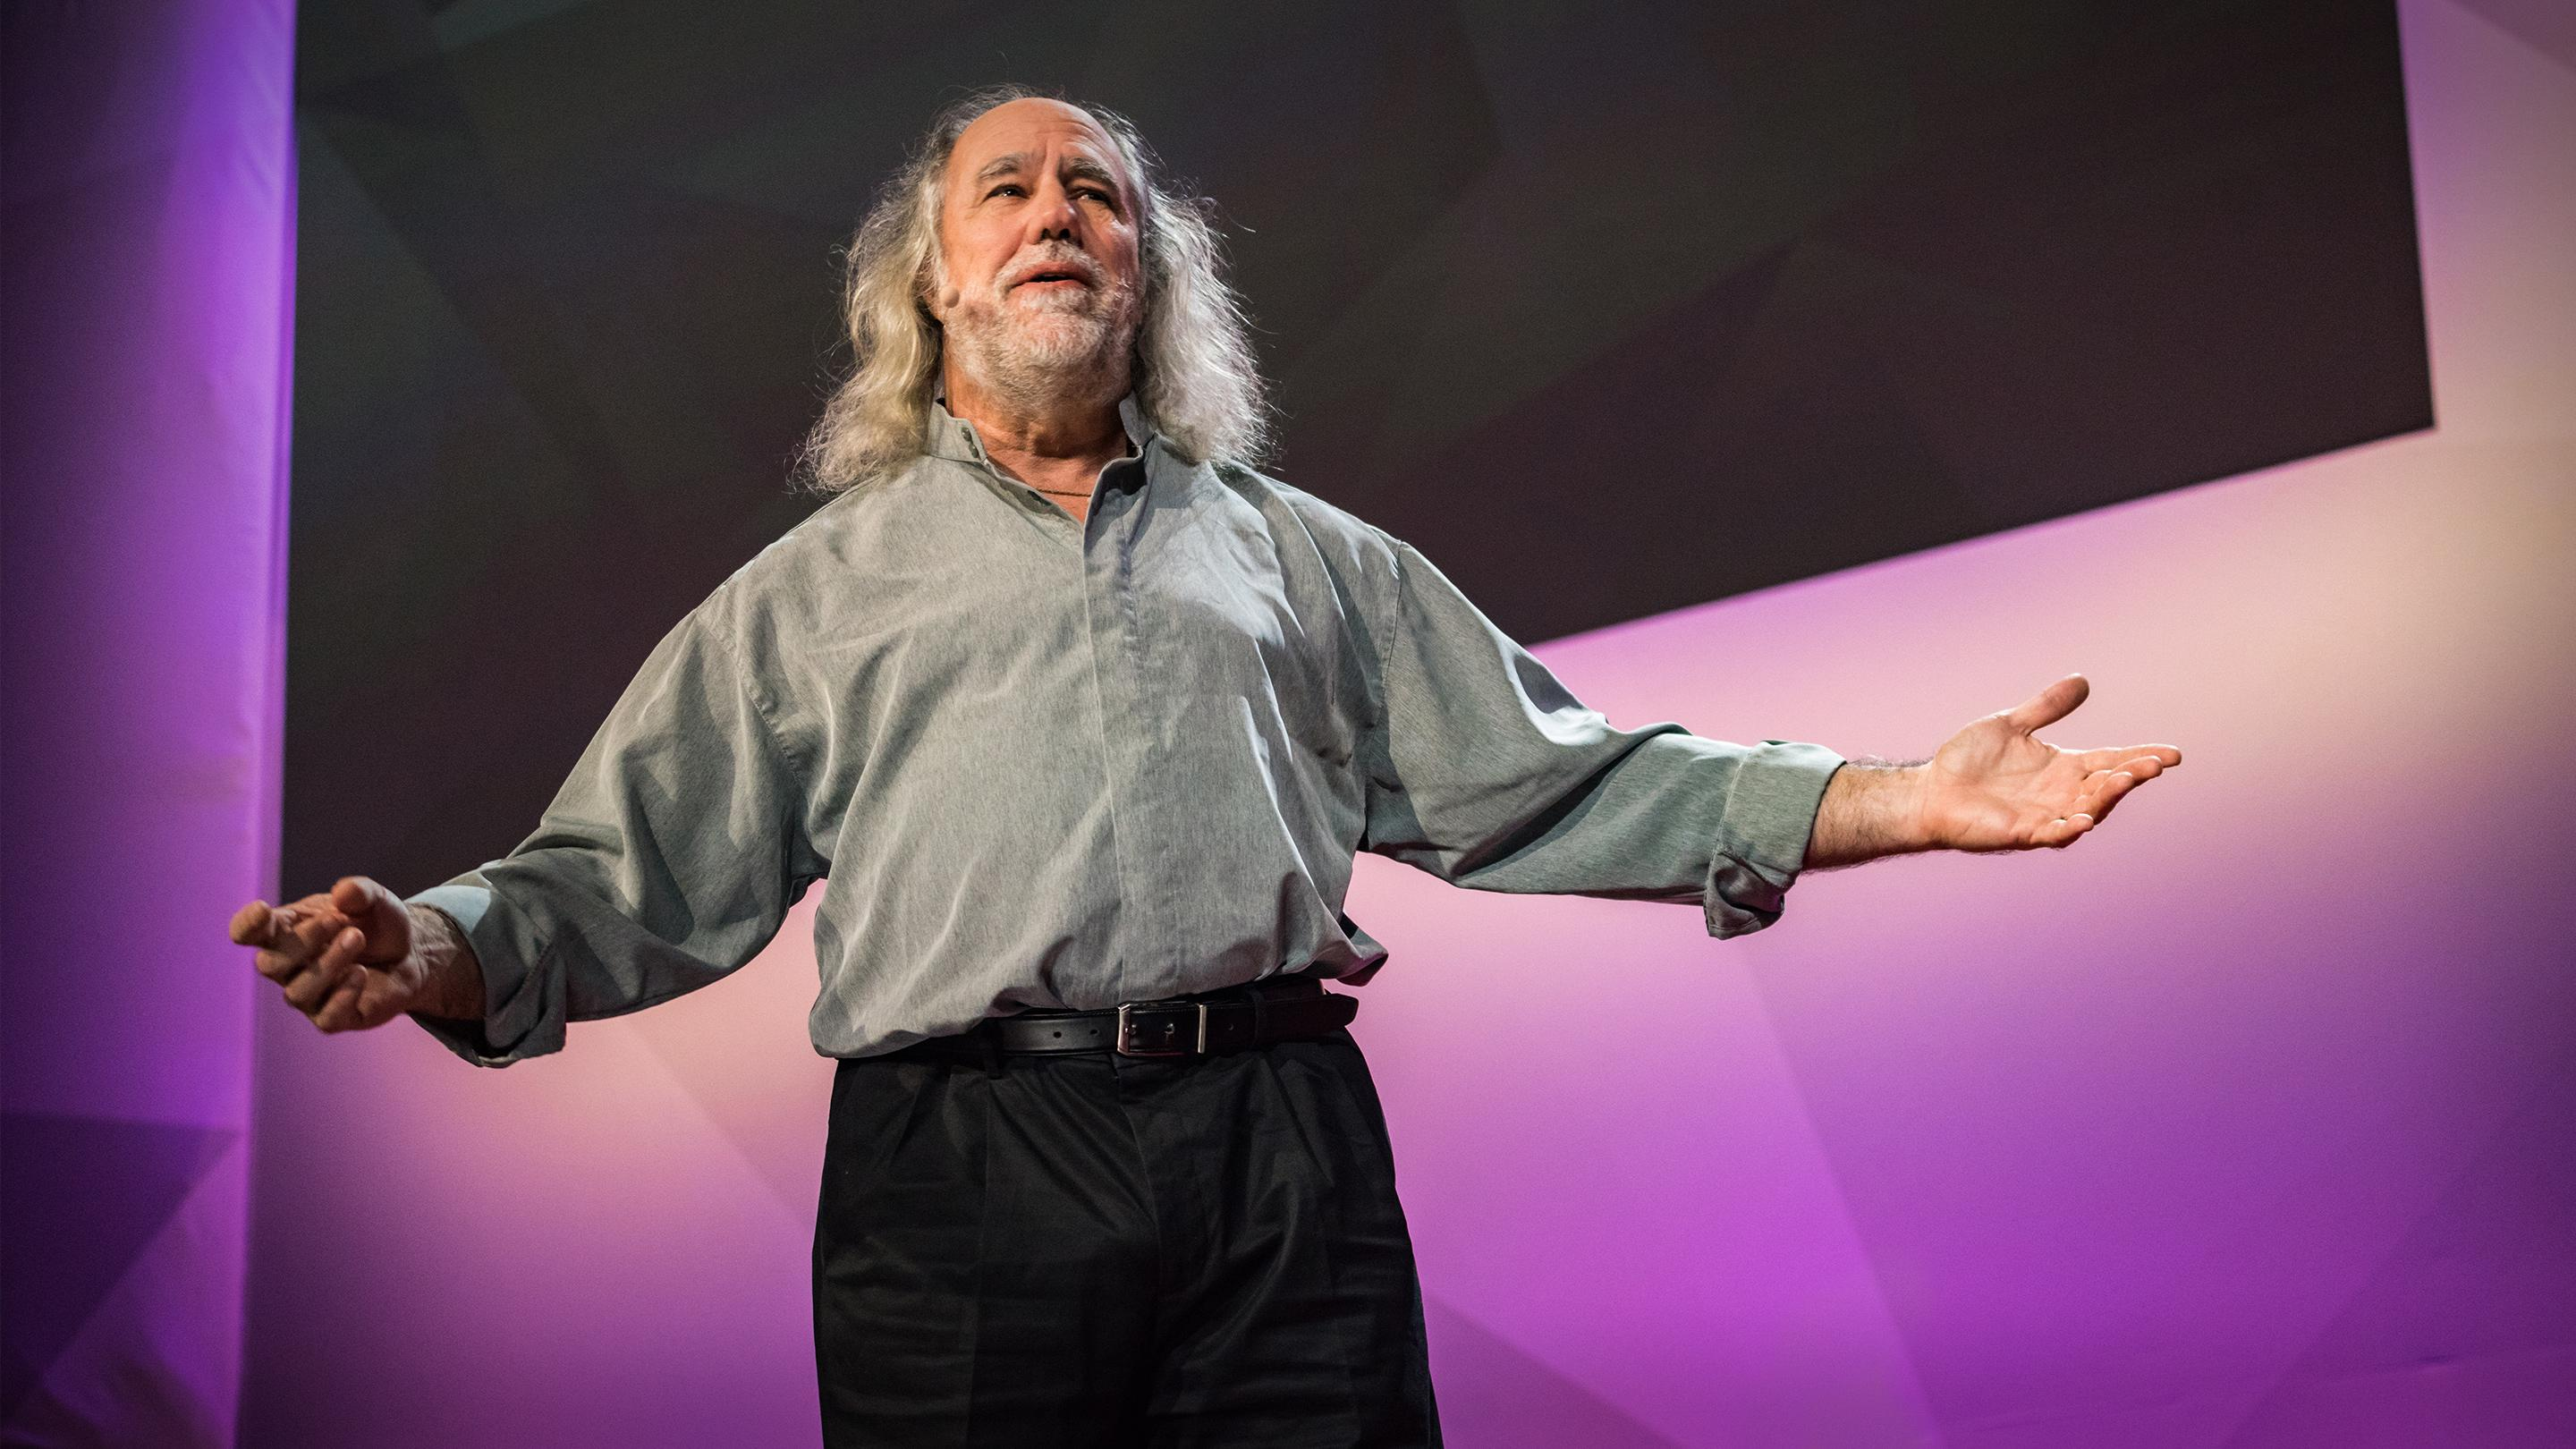
\includegraphics[width=\paperwidth]{grady-booch.jpg}
      };
    \end{tikzpicture}
  \end{frame}
}

{ % all template changes are local to this group.
  \setbeamertemplate{navigation symbols}{}
  \begin{frame}[plain]
    \begin{tikzpicture}[remember picture,overlay]
      \node[at=(current page.center)] {
        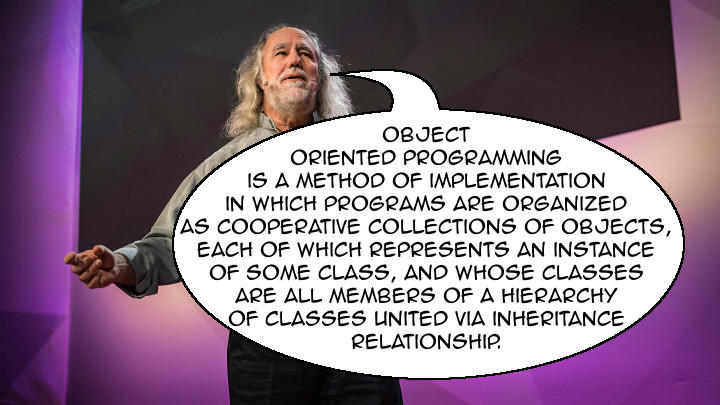
\includegraphics[width=\paperwidth]{grady-booch-oop.jpg}
      };
    \end{tikzpicture}
  \end{frame}
}

\begin{frame}{The four pillars of OOP}
  \begin{tabularx}{\textwidth}{ X X }
    \textbf{``Pillars'':} \pause \newline
    \begin{itemize}
    \item abstraction \pause
    \item encapsulation \pause
    \item inheritance \pause
    \item polymorphism \pause
    \end{itemize}
    &
    \textbf{Principles (Booch et al.)}: \pause \newline
    \begin{itemize}
    \item abstraction \pause
    \item encapsulation \pause
    \item modularity \pause
    \item hierarchy
    \end{itemize}
  \end{tabularx}
\end{frame}

\begin{frame}{The four pillars of OOP}
  \begin{tabularx}{\textwidth}{ X X }
    \textbf{``Pillars'':} \newline
    \begin{itemize}
    \item abstraction
    \item \sout{encapsulation}
    \item inheritance
    \item \sout{polymorphism}
    \end{itemize}
    &
    \textbf{Principles (Booch et al.)}: \newline
    \begin{itemize}
    \item abstraction
    \item \sout{encapsulation}
    \item \sout{modularity}
    \item \sout{hierarchy}
    \end{itemize}
  \end{tabularx}
\end{frame}


%\subsection{Abstraction}

{ % all template changes are local to this group.
  \setbeamertemplate{navigation symbols}{}
  \begin{frame}[plain]
    \begin{tikzpicture}[remember picture,overlay]
      \node[at=(current page.center)] {
        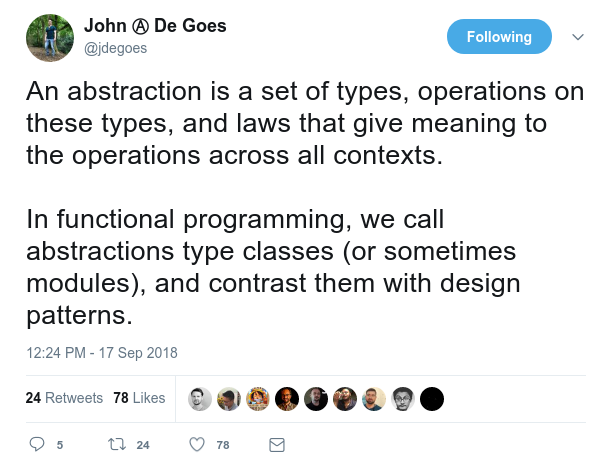
\includegraphics[width=\paperwidth]{degoes.png}
      };
    \end{tikzpicture}
  \end{frame}
}

{ % all template changes are local to this group.
  \setbeamertemplate{navigation symbols}{}
  \begin{frame}[plain]
    \begin{tikzpicture}[remember picture,overlay]
      \node[at=(current page.center)] {
        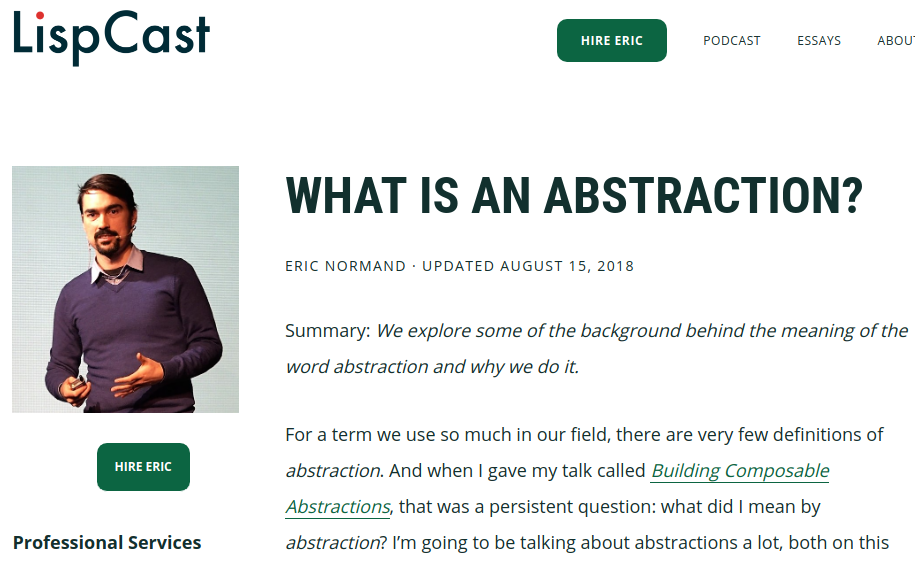
\includegraphics[width=\paperwidth]{normand-abst.png}
      };
    \end{tikzpicture}
  \end{frame}
}

{ % all template changes are local to this group.
  \setbeamertemplate{navigation symbols}{}
  \begin{frame}[plain]
    \begin{tikzpicture}[remember picture,overlay]
      \node[at=(current page.center)] {
        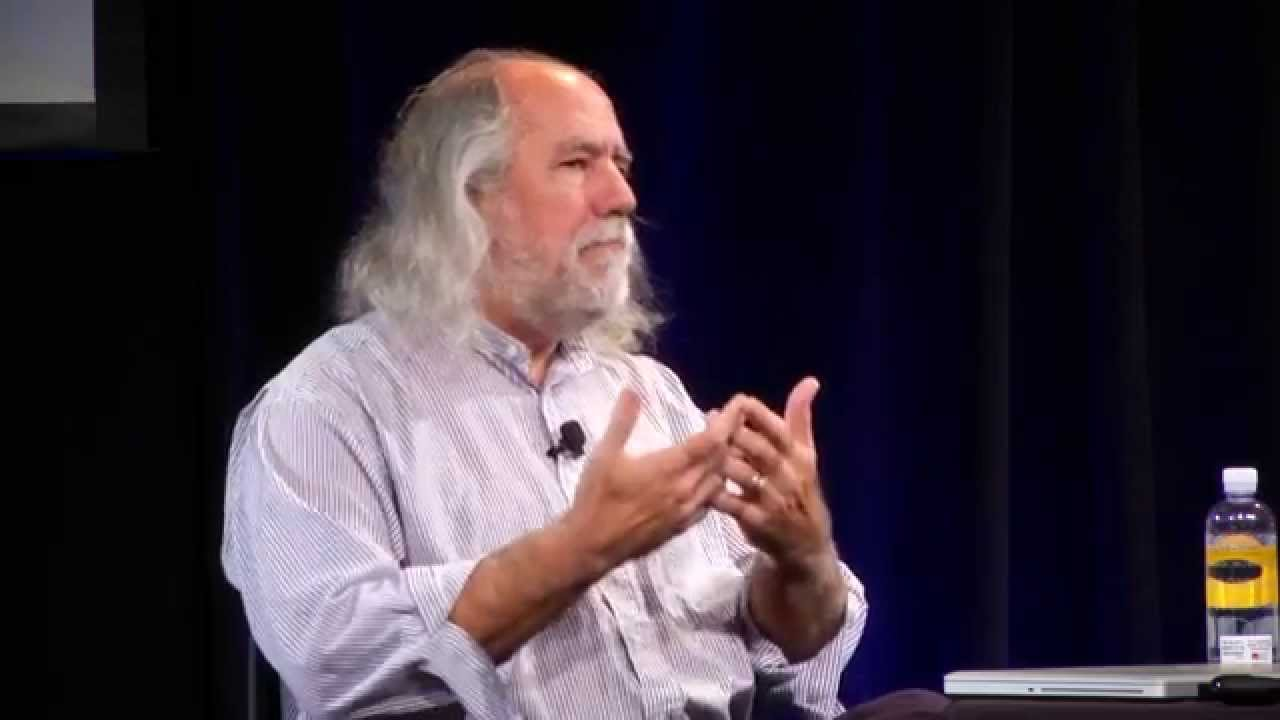
\includegraphics[width=\paperwidth]{grady-booch-explaining.jpg}
      };
    \end{tikzpicture}
  \end{frame}
}

{ % all template changes are local to this group.
  \setbeamertemplate{navigation symbols}{}
  \begin{frame}[plain]
    \begin{tikzpicture}[remember picture,overlay]
      \node[at=(current page.center)] {
        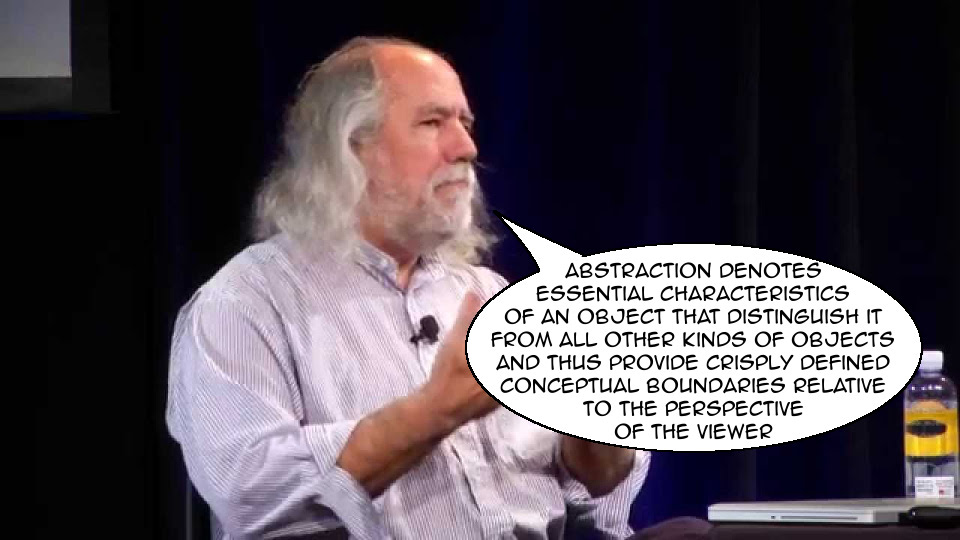
\includegraphics[width=\paperwidth]{grady-booch-abstraction.jpg}
      };
    \end{tikzpicture}
  \end{frame}
}

{ % all template changes are local to this group.
  \setbeamertemplate{navigation symbols}{}
  \begin{frame}[plain]
    \begin{tikzpicture}[remember picture,overlay]
      \node[at=(current page.center)] {
        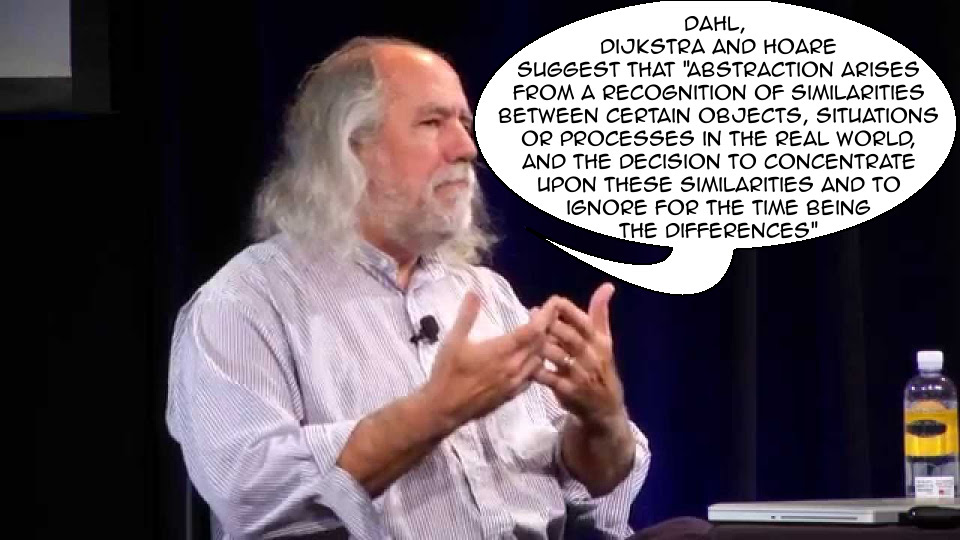
\includegraphics[width=\paperwidth]{grady-booch-dijkstra.jpg}
      };
    \end{tikzpicture}
  \end{frame}
}

{ % all template changes are local to this group.
  \setbeamertemplate{navigation symbols}{}
  \begin{frame}[plain]
    \begin{tikzpicture}[remember picture,overlay]
      \node[at=(current page.center)] {
        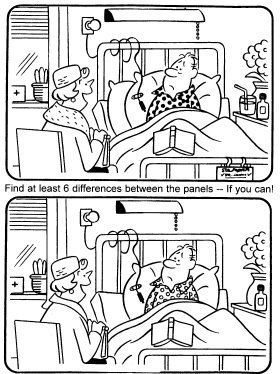
\includegraphics[width=0.3\paperwidth]{diff.jpeg}
      };
    \end{tikzpicture}
  \end{frame}
}

{ % all template changes are local to this group.
  \setbeamertemplate{navigation symbols}{}
  \begin{frame}[plain]
    \begin{tikzpicture}[remember picture,overlay]
      \node[at=(current page.center)] {
        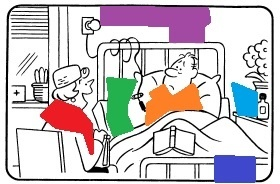
\includegraphics[width=0.3\paperwidth]{abstract.jpeg}
      };
    \end{tikzpicture}
  \end{frame}
}


%
{ % all template changes are local to this group.
  \setbeamertemplate{navigation symbols}{}
  \begin{frame}[plain]
    \begin{tikzpicture}[remember picture,overlay]
      \node[at=(current page.center)] {
        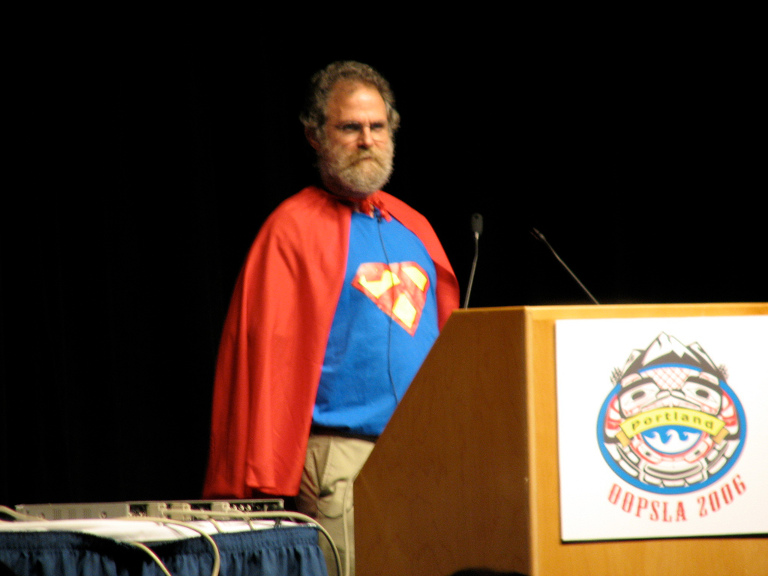
\includegraphics[height=\paperheight]{phil_wadler0.jpg}
      };
    \end{tikzpicture}
  \end{frame}
}

{ % all template changes are local to this group.
  \setbeamertemplate{navigation symbols}{}
  \begin{frame}[plain]
    \begin{tikzpicture}[remember picture,overlay]
      \node[at=(current page.center)] {
        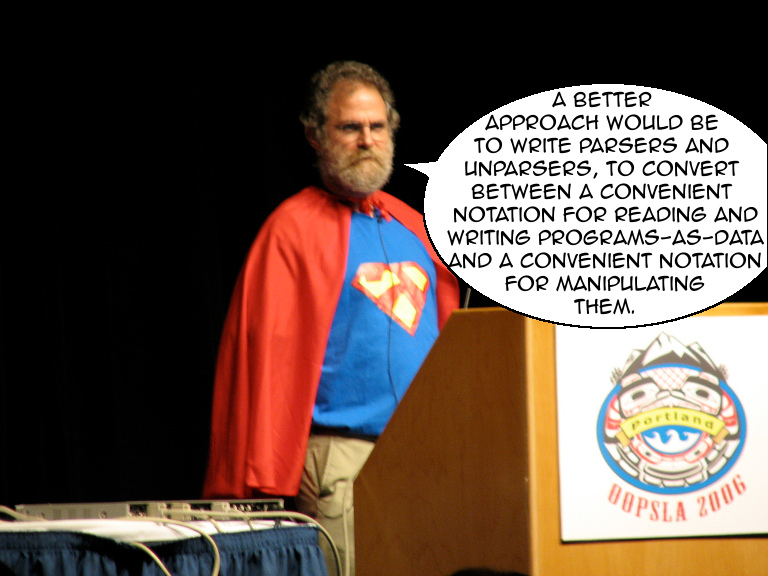
\includegraphics[height=\paperheight]{phil_wadler1.jpg}
      };
    \end{tikzpicture}
  \end{frame}
}

{ % all template changes are local to this group.
  \setbeamertemplate{navigation symbols}{}
  \begin{frame}[plain]
    \begin{tikzpicture}[remember picture,overlay]
      \node[at=(current page.center)] {
        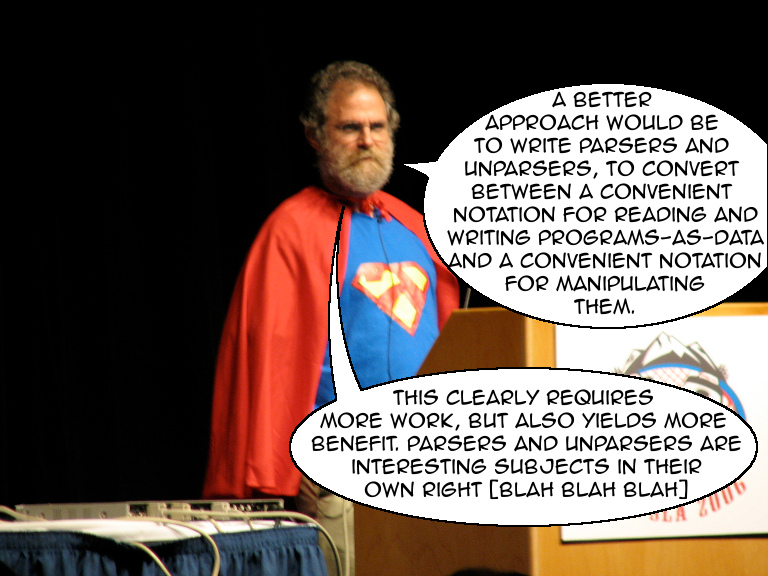
\includegraphics[height=\paperheight]{phil_wadler2.jpg}
      };
    \end{tikzpicture}
  \end{frame}
}



\end{document}
